%% LyX 2.2.0 created this file.  For more info, see http://www.lyx.org/.
%% Do not edit unless you really know what you are doing.
\documentclass[12pt,a4paper,ngerman,intoc,bibliography=totoc,index=totoc,BCOR7.5mm,captions=tableheading,titlepage,dvipsnames]{scrbook}
\usepackage{lmodern}
\renewcommand{\sfdefault}{lmss}
\renewcommand{\ttdefault}{lmtt}
\usepackage[T1]{fontenc}
\usepackage[latin9]{inputenc}
\setcounter{secnumdepth}{3}
\setlength{\parskip}{\medskipamount}
\setlength{\parindent}{0pt}
\usepackage{color}
\definecolor{note_fontcolor}{rgb}{0, 0, 1}
\usepackage{babel}
\usepackage{array}
\usepackage{float}
\usepackage{textcomp}
\usepackage{amsmath}
\usepackage{amssymb}
\usepackage{graphicx}
\usepackage[unicode=true,
 bookmarks=true,bookmarksnumbered=true,bookmarksopen=true,bookmarksopenlevel=1,
 breaklinks=true,pdfborder={0 0 1},backref=false,colorlinks=true]
 {hyperref}
\hypersetup{pdftitle={OpenSlides Handbuch},
 pdfauthor={OpenSlides Team},
 pdfsubject={OpenSlides Handbuch},
 pdfkeywords={OpenSlides Handbuch},
 linkcolor=black, citecolor=black, urlcolor=blue, filecolor=blue, pdfpagelayout=OneColumn, pdfnewwindow=true, pdfstartview=XYZ, plainpages=false}

\makeatletter

%%%%%%%%%%%%%%%%%%%%%%%%%%%%%% LyX specific LaTeX commands.
\pdfpageheight\paperheight
\pdfpagewidth\paperwidth

\newcommand{\noun}[1]{\textsc{#1}}
\DeclareRobustCommand*{\lyxarrow}{%
\@ifstar
{\leavevmode\,$\triangleleft$\,\allowbreak}
{\leavevmode\,$\triangleright$\,\allowbreak}}
%% Because html converters don't know tabularnewline
\providecommand{\tabularnewline}{\\}
%% The greyedout annotation environment
\newenvironment{lyxgreyedout}
  {\textcolor{note_fontcolor}\bgroup\ignorespaces}
  {\ignorespacesafterend\egroup}

%%%%%%%%%%%%%%%%%%%%%%%%%%%%%% Textclass specific LaTeX commands.
\newcommand{\code}[1]{\texttt{#1}}

\@ifundefined{date}{}{\date{}}
%%%%%%%%%%%%%%%%%%%%%%%%%%%%%% User specified LaTeX commands.
% Linkfl�che f�r Querverweise vergr��ern und automatisch benennen,
\AtBeginDocument{\renewcommand{\ref}[1]{\mbox{\autoref{#1}}}}
\@ifpackageloaded{babel}{
 \addto\extrasngerman{%
  \renewcommand*{\equationautorefname}[1]{}%
  \renewcommand{\sectionautorefname}{Kap.\negthinspace}%
  \renewcommand{\subsectionautorefname}{Kap.\negthinspace}%
  \renewcommand{\subsubsectionautorefname}{Kap.\negthinspace}%
 }
}{}


% provides caption formatting
\usepackage[labelfont={bf,sf}]{caption}[2004/07/16]

% enables calculation of values,
\usepackage{calc}

% increase the bottom float placement fraction
\renewcommand{\bottomfraction}{0.5}

% avoids that floats are placed before their
% corresponding section starts
\let\mySection\section\renewcommand{\section}{\suppressfloats[t]\mySection}

% used to have extra space in table cells
\@ifundefined{extrarowheight}
 {\usepackage{array}}{}
\setlength{\extrarowheight}{2pt}

\makeatother

\begin{document}

\title{\noun{OpenSlides} Handbuch}

\author{vom \noun{OpenSlides} Team\thanks{Wenn Sie Anmerkungen haben oder Fehler gefunden haben, senden Sie
bitte eine Mail an die deutsche Dokumentations-Mailingliste: \protect\href{mailto:users-de@openslides.org?subject=OpenSlides Handbuch}{users-de@openslides.org}\protect \\
Dazu m�ssen Sie sich vorher \protect\href{http://mail.openslides.org/listinfo/users-de/}{an der Liste anmelden}.}\\
\\
f�r \noun{OpenSlides} Version 2.0}

\maketitle
\tableofcontents{}

\include{OpenSlides-Einf�hrung}

%% LyX 2.2.0 created this file.  For more info, see http://www.lyx.org/.
%% Do not edit unless you really know what you are doing.
\documentclass[12pt,a4paper,ngerman,bibliography=totoc,index=totoc,BCOR7.5mm,titlepage,captions=tableheading,dvipsnames,table]{scrbook}
\usepackage{lmodern}
\renewcommand{\sfdefault}{lmss}
\renewcommand{\ttdefault}{lmtt}
\usepackage[T1]{fontenc}
\usepackage[latin9]{inputenc}
\setcounter{secnumdepth}{3}
\setlength{\parskip}{\medskipamount}
\setlength{\parindent}{0pt}
\usepackage{color}
\definecolor{note_fontcolor}{rgb}{0, 0, 1}
\usepackage{babel}
\usepackage{amsmath}
\usepackage{amssymb}
\usepackage{graphicx}
\usepackage[unicode=true,
 bookmarks=true,bookmarksnumbered=true,bookmarksopen=true,bookmarksopenlevel=2,
 breaklinks=true,pdfborder={0 0 1},backref=false,colorlinks=true]
 {hyperref}
\hypersetup{pdftitle={OpenSlides Handbuch},
 pdfauthor={OpenSlides Team},
 pdfsubject={OpenSlides Handbuch},
 pdfkeywords={OpenSlides, Handbuch},
 linkcolor=black, citecolor=black, urlcolor=blue, filecolor=blue, pdfpagelayout=OneColumn, pdfnewwindow=true, pdfstartview=XYZ, plainpages=false}

\makeatletter

%%%%%%%%%%%%%%%%%%%%%%%%%%%%%% LyX specific LaTeX commands.
\pdfpageheight\paperheight
\pdfpagewidth\paperwidth

\newcommand{\noun}[1]{\textsc{#1}}
%% The greyedout annotation environment
\newenvironment{lyxgreyedout}
  {\textcolor{note_fontcolor}\bgroup\ignorespaces}
  {\ignorespacesafterend\egroup}

%%%%%%%%%%%%%%%%%%%%%%%%%%%%%% Textclass specific LaTeX commands.
\newcommand{\code}[1]{\texttt{#1}}

\@ifundefined{date}{}{\date{}}
%%%%%%%%%%%%%%%%%%%%%%%%%%%%%% User specified LaTeX commands.
% that links to image floats jumps
% to the beginning of the float and 
% not to its caption
\usepackage[figure]{hypcap}

% the pages of the TOC is numbered roman
% and a PDF-bookmark for the TOC is added
\let\myTOC\tableofcontents
\renewcommand\tableofcontents{%
  \frontmatter
  \pdfbookmark[1]{\contentsname}{}
  \myTOC
  \mainmatter }

% Linkfl�che f�r Querverweise vergr��ern und automatisch benennen,
\AtBeginDocument{\renewcommand{\ref}[1]{\mbox{\autoref{#1}}}}
\@ifpackageloaded{babel}{
 \addto\extrasngerman{%
  \renewcommand*{\equationautorefname}[1]{}%
  \renewcommand{\sectionautorefname}{Kap.\negthinspace}%
  \renewcommand{\subsectionautorefname}{Kap.\negthinspace}%
  \renewcommand{\subsubsectionautorefname}{Kap.\negthinspace}%
 }
}{}

% provides caption formatting
\usepackage[labelfont={bf,sf}]{caption}[2004/07/16]

% enables calculation of values,
\usepackage{calc}

% increase the bottom float placement fraction
\renewcommand{\bottomfraction}{0.5}

% avoids that floats are placed before their
% corresponding section starts
\let\mySection\section\renewcommand{\section}{\suppressfloats[t]\mySection}

% used to have extra space in table cells
\@ifundefined{extrarowheight}
 {\usepackage{array}}{}
\setlength{\extrarowheight}{2pt}

\makeatother

\begin{document}

\chapter{Erste Schritte}

In diesem Kapitel werden die ersten Schritte bei \noun{OpenSlides}
erkl�rt.

\section{Installation\label{sec:Installation}}

\noun{OpenSlides} muss nur auf einem Computer installiert werden.
Dieser fungiert im Netzwerk als Server. Im Pr�sentationsmodus Single
gibt es kein Netzwerk. \noun{OpenSlides} muss dann auf dem einen
verwendeten Computer installiert werden.

Die aktuelle Version von \noun{OpenSlides}, f�r die dieses Handbuch
g�ltig ist, ist Version 2.0.

\subsection{Verwendung der Windows-Version (Portable Version mit openslides.exe)}

Laden Sie die aktuelle \noun{OpenSlides} Version f�r Windows von
\href{http://openslides.org}{http://openslides.org} herunter. Extrahieren
Sie das zip-Archiv (z. B. \code{openslides-N.N-portable.zip}) in
einen beliebigen Ordner. \noun{OpenSlides} muss nun nicht weiter
installiert werden. Alle notwendigen Programmelemente sind in dem
Ordner enthalten.

\subsection{Verwendung der Linux/MacOS-Version}

Laden Sie die aktuelle \noun{OpenSlides} Version f�r Linux/MacOS
von\\
\href{http://openslides.org}{http://openslides.org} oder �ber den
Python Package Index (PyPI) (\code{\$ pip install openslides}) herunter.
Die Installationsanleitung f�r diese Version finden Sie in der beiliegenden
README.rst. Folgen Sie den Anweisungen der Anleitung. 

\section{Konfiguration}

Nach der Installation ist \noun{OpenSlides} bereits vorkonfiguriert.
Die beim ersten Start erzeugte (leere) Datenbank enth�lt einige Voreinstellungen.
Die Konfiguration kann im laufenden Programm unter dem Tab \quotedblbase Konfiguration\textquotedblleft{}
vorgenommen werden. Weitere Einstellungsm�glichkeiten f�r erfahrene
Benutzer sind in der Datei \code{settings.py} m�glich. Diese Datei
liegt nicht im extrahierten \noun{OpenSlides} Verzeichnis, sondern
in einem Benutzerverzeichnis, das abh�ngig von Ihrem Betriebssystem
ist. Unter Windows (au�er bei der Portable Version) ist es standardm��ig

\code{\$HOME\textbackslash{}AppData\textbackslash{}Local\textbackslash{}openslides}

, unter Linux/MacOS ist es standardm��ig

\code{\textasciitilde{}/.config/openslides}

\section{Start des Servers und �ffnen des Browsers\label{sec:Start-des-Servers}}

\subsection{Verwendung der Windows-Version (Portable Version mit openslides.exe)}

Wenn Sie die Windows-Version (Portable Version mit openslides.exe)
verwenden, brauchen Sie nur die Datei \code{openslides.exe} auszuf�hren.
Mit dieser wird der eine grafische Oberfl�che gestartet, mit der Sie
den \noun{OpenSlides}-Server konfigurieren, starten und jederzeit
beenden k�nnen:

\begin{center}
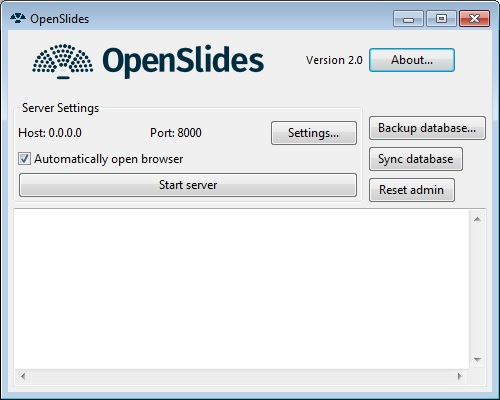
\includegraphics[scale=0.7]{clipart/OpenSlides-Server-before-Start}
\par\end{center}

Zum Starten klicken Sie einfach auf den Knopf \textsf{Start~server}
und ihr Webbrowser �ffnet sich.

Falls Sie Ihren Administrator-Zugang vergessen haben, k�nnen Sie mit
Klick auf \textsf{Reset~admin} einen neuen Admin-Nutzer erstellen,
dessen Name und Passwort. \textsf{admin} ist.

In \textsf{Settings} k�nnen Sie optional den Webhost und Port einstellen;
mehr dazu siehe ??. Mit \textsf{Backup~database} und \textsf{Sync~database}
k�nnen Sie Sitzungen speichern bzw.\ laden; mehr dazu siehe ??.

\subsection{Verwendung der Linux/MacOS-Version}

Starten Sie den Server, indem Sie in der Kommandozeile eingeben:

\code{\$ openslides}

Wenn Sie eine virtuelle Arbeitsumgebung (virtualenv) verwenden, m�ssen
Sie diese zuvor aktivieren:

\code{\$ source .venv/bin/activate}

Damit wird der Server gestartet und ihr Browser mit der richtigen
URL ge�ffnet.

\noun{OpenSlides} kann jederzeit im Fenster der Kommandozeile mit
der Tastenkombination \textsf{Strg+C} beendet werden. Alle eingegebenen
Daten bleiben in der Datenbank gespeichert.

Weitere Startoptionen k�nnen Sie mit folgender Eingabe sehen:

\code{\$ openslides \textendash help}

\subsection{�ffnen des Browsers}

Bei Start des Servers wird automatisch der Browser mit der richtigen
URL ge�ffnet.

Falls dies wegen Ihrer Browsereinstellungen nicht gelingt, rufen Sie
das \noun{OpenSlides}-Webinterface auf, indem Sie in die Adresszeile
die IP-Adresse des Servers eintragen. Sie hat oft die Form \code{http://192.168.x.y/},
wobei x und y f�r eine bestimmte Zahl mit ein bis drei Ziffern stehen.
Am Computer, auf dem \noun{OpenSlides} gestartet wurde, kann \noun{OpenSlides}
auch �ber \code{http://localhost:8000} aufgerufen werden.

\subsection{Erster Login}

Der erste Login als Administrator ist mit dem Benutzernamen \textsf{admin}
und dem Passwort \textsf{admin} m�glich. Sie sollten das Passwort
nach dem ersten Start �ndern, siehe \ref{subsec:Benutzername-oder-Passwort},
um Unbefugten keinen Zugriff auf Ihre Daten zu gew�hren.

\begin{lyxgreyedout}
\textbf{Hinweis:} \noun{OpenSlides} ben�tigt Cookies um die Identit�t
des Nutzers festzustellen, solange er eingeloggt ist. Beim Ausloggen
wird das Cookie wieder gel�scht.%
\end{lyxgreyedout}

\newpage{}

\section{Arbeiten mit \protect\noun{OpenSlides}}

Nach dem ersten Einloggen sieht \noun{OpenSlides} so aus:

\begin{center}
\includegraphics[width=1\columnwidth]{clipart/�bersicht-nach-Start}
\par\end{center}

In der Kopfzeile kann man durch Klicken auf das Logo jederzeit auf
die Startseite zur�ckkehren. In der Zeile rechts k�nnen Sie mit anderen
Nutzern chatten, siehe ??, Ihr Profile bearbeiten und ihr Passwort
�ndern, siehe \ref{sec:An--und-Abmelden} und die Men�sprache von
\noun{OpenSlides} �ndern.

In der Men�leiste k�nnen Sie �ber die Men�punkte alle Inhalte in \noun{OpenSlides}
eingeben und verwalten.

\begin{center}
\includegraphics[width=1\columnwidth]{clipart/Men�leiste}
\par\end{center}
\begin{itemize}
\item Im Men�punkt \textbf{Startseite} k�nnen Sie die Teilnehmer willkommen
hei�en und kurz erkl�ren, wie man \noun{OpenSlides} nutzt.
\item Im Men�punkt \textbf{Tagesordnung} k�nnen Sie die Tagesordnung der
Veranstaltung im Vorfeld oder live anlegen, entsprechende Folien vorbereiten
und die Rednerliste verwalten. Mehr zur Tagesordnung siehe \ref{sec:Tagesordnung}.
\item Unter \textbf{Antr�ge} verwalten Sie die gestellten Antr�ge und die
dazugeh�rigen Abstimmungen. Mehr dazu siehe \ref{sec:Antr=0000E4ge}.
\item Der Punkt \textbf{Wahlen} verwaltet die Wahl�mter mit den Kandidaten
sowie die jeweiligen Wahlergebnisse. Mehr zur dazu siehe \ref{sec:Wahlen}.
\item Der Men�punkt \textbf{Teilnehmer/innen} erm�glicht einen Zugriff auf
die Personenprofile. Mehr zur dazu siehe \ref{sec:Teilnehmer}.
\item Unter dem Punkt \textbf{Dateien} k�nnen Sie eigene Dateien auf den
Server laden und zum Download anbieten. PDF-Dateien k�nnen auch auf
dem Projektor angezeigt werden. Mehr zur dazu siehe \ref{sec:Dateien}.
\item Im Men�punkt \textbf{Einstellungen} k�nnen die grundlegenden Einstellungen
f�r die Veranstaltung vorgenommen werden. Mehr zur dazu siehe \ref{sec:Einstellungen-=0000DCbersicht}.
\end{itemize}
Wenn Sie auf das Symbol 
\includegraphics[scale=0.5]{clipart/Projektorsymbol-Leiste}
klicken, wird neben dem Begr��ungstext der aktuell projizierte Inhalt
angezeigt (Live-Vorschau):

\begin{center}
\includegraphics[width=1\columnwidth]{clipart/�bersicht-nach-Start-Projektor}
\par\end{center}

Damit haben Sie immer im Blick was die Teilnehmer gerade sehen und
k�nnen w�hrend der Sitzung arbeiten. Das Projektorbild in voller Gr��e
bekommen Sie in einem neuen Browsertab zu sehen, indem Sie auf die
Live-Vorschau klicken. Sie ist auch unter der URL \code{/projector/}
zu finden. Loggen Sie sich an dem Computer, an dem der Projektor angeschlossen
ist, in \noun{OpenSlides} ein und rufen Sie den Link oder die URL
auf. Legen Sie die Anzeige in einem eigenen Browserfenster auf den
Projektor und projizieren Sie sie so auf die Leinwand. In vielen Browsern
kann mit der Taste \textsf{F11} in den Vollbildmodus gewechselt werden.
Im \emph{Pr�sentationsmodus Single} m�ssen Sie die Bildschirmanzeige
auf Erweiterung/erweiterter Desktop stellen und das Browserfenster
mit dem Projektorbild auf den Projektor schieben.

Das Projektorbild aktualisiert sich vollkommen automatisch. Sollte
die Aktualisierung auf Grund eines Fehlers, zum Beispiel einer Unterbrechung
der Verbindung zum Server, aussetzen, kann das Projektorbild an dem
Computer, an dem der Projektor angeschlossen ist, regelm��ig mit der
Taste \textsf{F5} zur�ckgesetzt werden. Um dem Kopf des Projektorfensters
nach einer �nderung in der Konfiguration zu aktualisieren, muss ebenfalls
das Browserfenster zur�ckgesetzt werden.

Unterhalb der Live-Vorschau gibt es die Rubriken \textsf{Countdown}
und \textsf{Mitteilungen}. Mehr dazu siehe \ref{sec:Countdown-und-Mitteilungen}.
\end{document}


%% LyX 2.2.0 created this file.  For more info, see http://www.lyx.org/.
%% Do not edit unless you really know what you are doing.
\documentclass[12pt,a4paper,ngerman,bibliography=totoc,index=totoc,BCOR7.5mm,titlepage,captions=tableheading,dvipsnames,table]{scrbook}
\usepackage{lmodern}
\renewcommand{\sfdefault}{lmss}
\renewcommand{\ttdefault}{lmtt}
\usepackage[T1]{fontenc}
\usepackage[latin9]{inputenc}
\setcounter{secnumdepth}{3}
\setlength{\parskip}{\medskipamount}
\setlength{\parindent}{0pt}
\usepackage{color}
\usepackage{babel}
\usepackage{amsmath}
\usepackage{amssymb}
\usepackage{graphicx}
\inputencoding{utf8}
\usepackage[unicode=true,
 bookmarks=true,bookmarksnumbered=true,bookmarksopen=true,bookmarksopenlevel=2,
 breaklinks=true,pdfborder={0 0 1},backref=false,colorlinks=true]
 {hyperref}
\hypersetup{pdftitle={Tutorium – Administration einer Versammlung},
 pdfauthor={OpenSlides Team},
 pdfsubject={OpenSlides Handbuch, Administration},
 pdfkeywords={OpenSlides, Handbuch, Tutorium, Administration, Versammlung},
 linkcolor=black, citecolor=black, urlcolor=blue, filecolor=blue, pdfpagelayout=OneColumn, pdfnewwindow=true, pdfstartview=XYZ, plainpages=false}
\inputencoding{latin9}

\makeatletter

%%%%%%%%%%%%%%%%%%%%%%%%%%%%%% LyX specific LaTeX commands.
\pdfpageheight\paperheight
\pdfpagewidth\paperwidth

\newcommand{\noun}[1]{\textsc{#1}}
\DeclareRobustCommand*{\lyxarrow}{%
\@ifstar
{\leavevmode\,$\triangleleft$\,\allowbreak}
{\leavevmode\,$\triangleright$\,\allowbreak}}

%%%%%%%%%%%%%%%%%%%%%%%%%%%%%% Textclass specific LaTeX commands.
\newcommand{\code}[1]{\texttt{#1}}

\@ifundefined{date}{}{\date{}}
%%%%%%%%%%%%%%%%%%%%%%%%%%%%%% User specified LaTeX commands.
% that links to image floats jumps
% to the beginning of the float and 
% not to its caption
\usepackage[figure]{hypcap}

% the pages of the TOC is numbered roman
% and a PDF-bookmark for the TOC is added
\let\myTOC\tableofcontents
\renewcommand\tableofcontents{%
  \frontmatter
  \pdfbookmark[1]{\contentsname}{}
  \myTOC
  \mainmatter }

% Linkfl�che f�r Querverweise vergr��ern und automatisch benennen,
\AtBeginDocument{\renewcommand{\ref}[1]{\mbox{\autoref{#1}}}}
\@ifpackageloaded{babel}{
 \addto\extrasngerman{%
  \renewcommand*{\equationautorefname}[1]{}%
  \renewcommand{\sectionautorefname}{Kap.\negthinspace}%
  \renewcommand{\subsectionautorefname}{Kap.\negthinspace}%
  \renewcommand{\subsubsectionautorefname}{Kap.\negthinspace}%
 }
}{}

% provides caption formatting
\usepackage[labelfont={bf,sf}]{caption}[2004/07/16]

% enables calculation of values,
\usepackage{calc}

% increase the bottom float placement fraction
\renewcommand{\bottomfraction}{0.5}

% avoids that floats are placed before their
% corresponding section starts
\let\mySection\section\renewcommand{\section}{\suppressfloats[t]\mySection}

% used to have extra space in table cells
\@ifundefined{extrarowheight}
 {\usepackage{array}}{}
\setlength{\extrarowheight}{2pt}

\makeatother

\begin{document}

\chapter{Tutorium \textendash{} Administration einer Versammlung}

Dieses Tutorial ist auf dem Stand von \noun{OpenSlides} 2.0.x.

In diesem Tutorial sehen Sie am Beispiel der Mitgliederversammlung
eines Kleingartenvereins, wie Sie \noun{OpenSlides} im Pr�sentationsmodus
bedienen.

Zun�chst lernen Sie, OpenSlides allgemein einzurichten und Folien
auf dem Projektor zu zeigen. Anschlie�end k�nnen Sie die einzelnen
Tutorials f�r Tagesordnung, Teilnehmerverwaltung, Antr�ge, Wahlen
und Dateien durcharbeiten.

Alle Tutorials gehen von folgenden Rahmenbedingungen aus:

Der Verein \quotedblbase Schreberverein Nord e.\,V.\textquotedblleft{}
h�lt am 2.~M�rz~2017 seine j�hrliche Mitgliederversammlung ab. Auf
der Versammlung werden verschiedene Berichte gehalten und �ber eine
Satzungs�nderung abgestimmt. Au�erdem finden Wahlen zum Vorstand und
zum Beirat statt.

Auf den n�chsten Seiten folgen die einzelnen Tutorials. 

\section{Einrichtung von \protect\noun{OpenSlides}}

Zun�chst m�ssen Sie \noun{OpenSlides} auf dem Server installieren,
den Server starten und einige Einstellungen f�r Ihre Veranstaltung
vornehmen. Danach k�nnen Sie Ihre ersten Folien einrichten und auf
dem Projektor zeigen.

\subsection{Installation und Start des Servers}

Installieren Sie \noun{OpenSlides} wie in \ref{sec:Installation}
beschrieben. Starten Sie anschlie�end den Server wie in \ref{sec:Start-des-Servers}
erl�utert. Sie sehen jetzt die Login-Seite von \noun{OpenSlides}
in Ihrem Browser. Loggen Sie sich als Administrator ein, indem Sie
als Benutzernamen \textsf{admin} und als Passwort \textsf{admin} eingeben
und auf \textsf{Anmelden} klicken.

\begin{center}
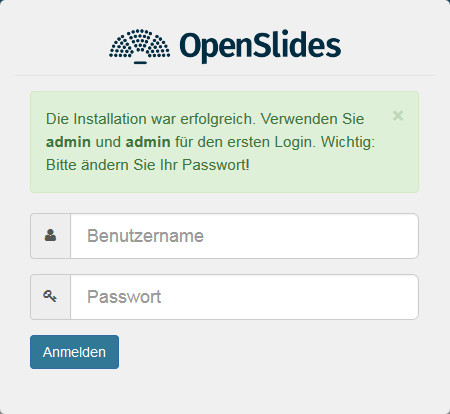
\includegraphics[width=0.74\columnwidth]{clipart/Login-Bildschirm}
\par\end{center}

Anschlie�end sollten Sie sofort das Administrator-Passwort �ndern.
Klicken Sie dazu oben rechts in der Kopfzeile


\includegraphics[scale=0.7]{clipart/Kopfzeile}

auf \textsf{Administrator} und dann auf \textsf{Passwort �ndern}.
Geben Sie in die entsprechenden Felder Ihr altes Passwort \textsf{admin}
und anschlie�end Ihr neues Passwort ein. Wiederholen Sie das neue
Passwort im dritten Formularfeld. Best�tigen Sie die Eingabe mit \textsf{Speichern}.
Weitere Informationen zur Benutzerverwaltung finden Sie in \ref{sec:An--und-Abmelden}. 

\subsection{Konfiguration des Systems}

Geben Sie die Rahmendaten Ihrer Veranstaltung ins System ein. Wechseln
Sie dazu zum Men�punkt \textsf{Einstellungen\lyxarrow{}Allgemein}
und geben Sie die Veranstaltungsdaten wie folgt ein:

\begin{center}
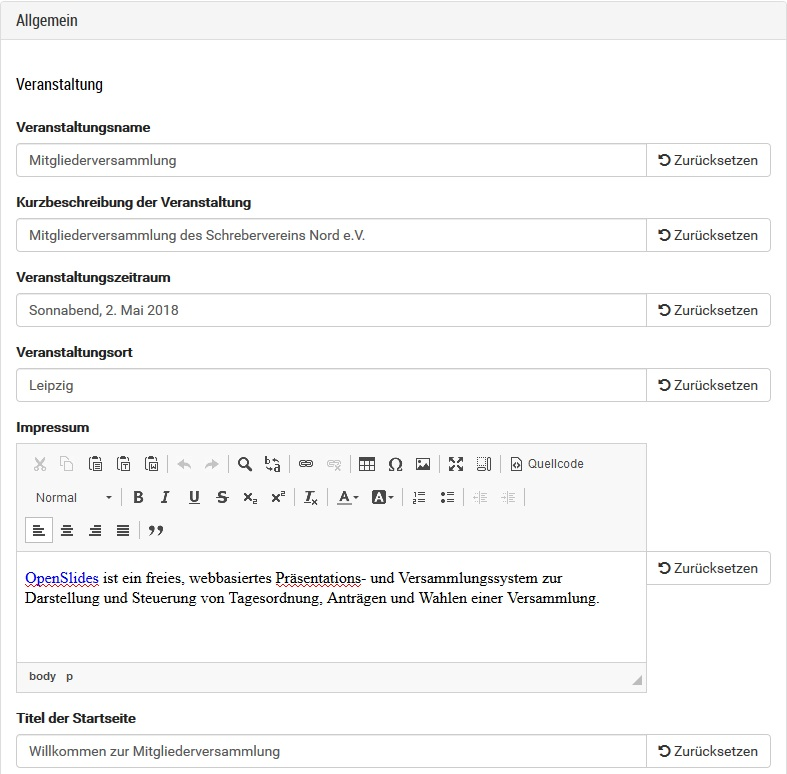
\includegraphics[width=1\columnwidth]{clipart/Einstellungen-Allgemein}
\par\end{center}

Das Impressum verweist voreingestellt auf \noun{OpenSlides}. Es erscheint
als Fu�zeile in der Startseite. Der Text im Feld \textsf{Diesen Text
auf der Login-Seite anzeigen} erscheint auf dem Login-Fenster, wenn
sich die Teilnehmer einloggen:

\begin{center}
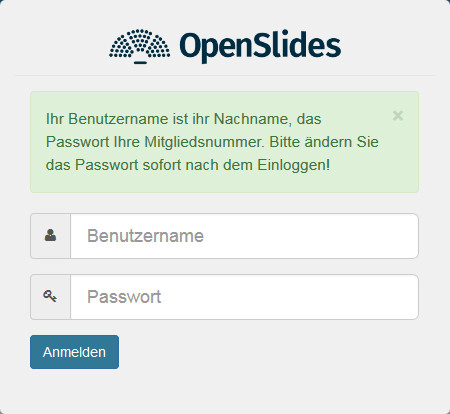
\includegraphics[width=0.74\columnwidth]{clipart/Login-Bildschirm-angepasst}
\par\end{center}

Alle �nderungen in den \textsf{Einstellungen} werden sofort gespeichert.
Alle Einstellungen sind im Detail in \ref{sec:Einstellungen-=0000DCbersicht}
beschrieben.

\subsection{Technische Einrichtung im Veranstaltungsraum}

Im Pr�sentationsmodus Single schlie�en Sie den Projektor an Ihren
Computer an und schieben ein zweites Browserfenster mit der Projektoransicht
auf den Projektor. In den anderen Modi richten Sie ein Netzwerk ein,
schlie�en Sie einen beliebigen Computer an den Projektor an und �ffnen
im Vollbildmodus die Seite mit der Projektoransicht. Die Projektoransicht
bekommen Sie in einem neuen Browsertab zu sehen, indem Sie auf die
Live-Vorschau klicken. Diese ist auch unter der URL \code{/projector/}
zu finden.

\newpage{}

\section{Tagesordnung verwalten}

In diesem Teil lernen Sie, wie Sie Eintr�ge in der Tagesordnung erstellen
und verwalten.

\subsection{Konfiguration der Tagesordnung}

Gehen Sie zun�chst im Men�punkt \textsf{Konfiguration\lyxarrow{}Tagesordnung\lyxarrow{}Allgemein}
zum Unterpunkt \textsf{Beginn der Veranstaltung}. Hier k�nnen Sie
den genauen Beginn der Veranstaltung einstellen. Zum Beispiel: \textsf{02.03.2017
10:00}

Die weiteren Einstellungen der Tagesordnung sind in \ref{subsec:Einstellungen-Tagesordnung}
beschrieben.

\subsection{Eingabe der Tagesordnung}

Die Tagesordnung enth�lt nach einer Neuinstallation noch keine Eintr�ge.
Legen Sie zun�chst einige Eintr�ge an. Klicken Sie dazu im Men�punkt
\textsf{Tagesordnung} oben rechts auf 
\includegraphics[scale=0.7]{clipart/Neu-Symbol}
und geben Sie einen Eintrag wie folgt ein:

\newpage{}

\begin{center}
\includegraphics[width=1\columnwidth]{clipart/TOP-erstellen-�ndern}
\par\end{center}

Wie sie sehen, k�nnen Sie den Text frei formatieren und dort auch
Bilder einf�gen. Im Feld \textsf{Anhang} k�nnen Sie aus allen in \noun{OpenSlides}
verf�gbaren Dateien einen Anhang w�hlen. Mehr zu Dateien ist in \ref{sec:Dateien}
beschrieben.\\
Klicken Sie abschlie�end auf \textsf{Speichern}.

Erweitern Sie nun die Tagesordnung um Eintr�ge mit folgenden Titeln:
\begin{itemize}
\item Bericht des Vorstands
\item Satzungs�nderung
\item Gartenfest
\item Sonstiges
\item Wahlen der Vereins�mter
\end{itemize}
Klicken Sie abschlie�end auf den Knopf 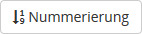
\includegraphics[scale=0.7]{clipart/Tagesordnung-nummerieren}
und die Tagesordnung wird nummeriert. Die �bersicht �ber die Eintr�ge
sieht nun so aus:

\begin{center}
\includegraphics[width=1\columnwidth]{clipart/Tagesordnung-�bersicht}
\par\end{center}

Sie k�nnen nun nachtr�glich die Reihenfolge der Eintr�ge ver�ndern
und auch Tagesordnungspunkte zu Unterpunkten verschieben. Klicken
Sie dazu oben auf den Knopf 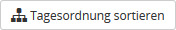
\includegraphics[scale=0.7]{clipart/Tagesordnung-sortieren}
und ziehen Sie dann mit gedr�ckter linker Maustaste den Punkt \textsf{Sonstiges}
an die letzte Stelle. Den Punkt \textsf{Gartenfest} ziehen Sie unter
\textsf{Bericht des Vorstands} und schieben ihn etwas nach rechts,
bis er dort einrastet. Gehen sie durch Dr�cken des Knopfes \includegraphics[scale=0.7]{clipart/Zur�ck-�bersicht}
zur�ck zu �bersicht und dr�cken Sie 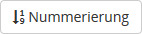
\includegraphics[scale=0.7]{clipart/Tagesordnung-nummerieren}
um die Nummerierung zu aktualisieren. Die �bersicht sieht nun so aus:

\newpage{}

\begin{center}
\includegraphics[width=1\columnwidth]{clipart/Tagesordnung-�bersicht-editiert}
\par\end{center}

\subsection{Einrichtung eigener Folien}

Eigene Folien werden verwendet, um Dinge au�erhalb der offiziellen
Tagesordnung zu behandeln. Technisch sind sie jedoch dasselbe wie
ein Tagesordnungspunkt.

Um z.\,B. den Teilnehmern mitzuteilen, dass es eine Kaffeepause gibt,
erstellen Sie einen neuen Tagesordnungspunkt:

\newpage{}

\begin{center}
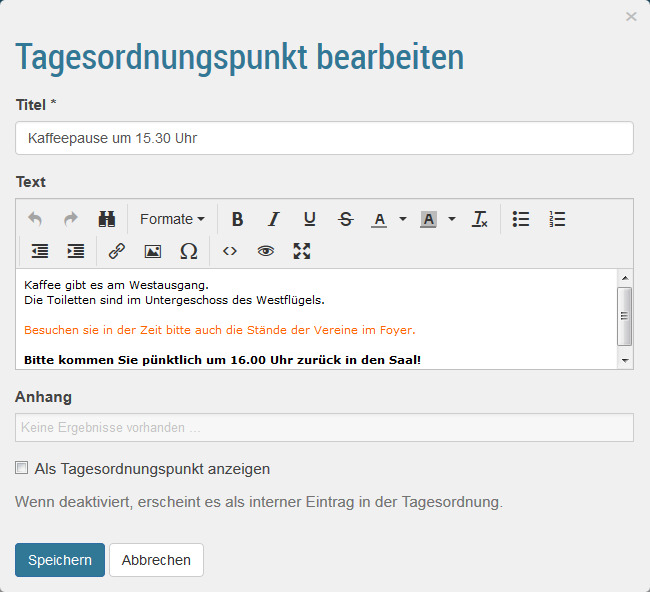
\includegraphics[width=1\columnwidth]{clipart/Eigene-Folie}
\par\end{center}

Dabei ist es wichtig, dass die Option \textsf{Als Tagesordnungspunkt
anzeigen} \emph{nicht} ausgew�hlt ist.

Eigene Folien werden in der �bersicht rosa unterlegt, um anzuzeigen,
dass sie nicht Teil der offiziellen Tagesordnung sind.

\subsection{Projektion der Tagesordnung}

Die komplette Tagesordnung wird projiziert, wenn Sie auf das Symbol\\

\includegraphics[scale=0.7]{clipart/Tagesordnung-projizieren} dr�cken.
Durch Dr�cken von \includegraphics[scale=0.7]{clipart/Untermen�-Symbol}
neben dem Symbol, k�nnen Sie w�hlen, ob alle Tagesordnungspunkte oder
nur die Hauptpunkte angezeigt werden, also in unserem Fall ohne den
Punkt \textsf{Gartenfreunde}. Eigene Folie werden in der Tagesordnung
nicht projiziert.

Einzelne Tagesordnungspunkte werden projiziert, indem Sie auf das
Symbol 
\includegraphics[scale=0.7]{clipart/Projektorsymbol} vor dem
entsprechenden Eintrag klicken. So k�nnen Sie eigene Folien projizieren.

\subsection{�ndern von Tagesordnungspunkten}

Der Inhalt von Tagesordnungspunkten kann jederzeit ge�ndert werden,
insbesondere w�hrend der Veranstaltung. Dazu zeigen sie mit der Maus
auf einen Tagesordnungspunkt und es erscheint ein Kontextmen�:

\begin{center}
\includegraphics[scale=0.95]{clipart/TOP-mit-Men�}
\par\end{center}

�ndern Sie zum Beispiel den Inhalt des Tagesordnungspunktes \textsf{Bericht
des Vorstandes}, indem Sie dort auf \textsf{Bearbeiten} klicken und
einen Text zum Tagesordnungspunkt eingeben.

Als Alternative f�r das Bearbeiten k�nnen Sie im Kontextmen� auf \textsf{Quick-Edit}
klicken und so oft ben�tigte Dinge wie die \textsf{Dauer} �ndern.

\begin{center}
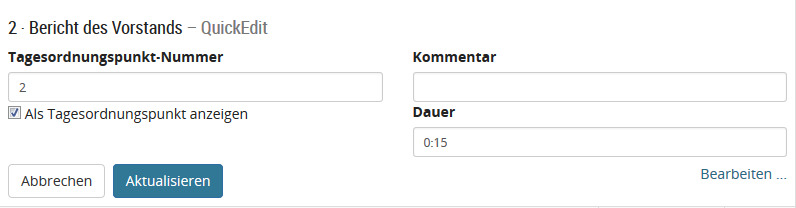
\includegraphics[width=1\columnwidth]{clipart/TOP-QuickEdit}
\par\end{center}

\subsection{Redelisten\label{subsec:Redelisten}}

\noun{OpenSlides} verf�gt bei jedem Tagesordnungseintrag �ber eine
Redelistenfunktion. Um eine Redeliste zu erstellen oder zu bearbeiten,
klicken Sie im Kontextmen� des jeweiligen Tagesordnungspunkts auf
\textsf{Redeliste}. Alternativ klicken Sie auf den Tagesordnungspunkt
und dann auf 
\includegraphics[scale=0.7]{clipart/Redeliste-Symbol}.

Setzen Sie sich selbst auf die Redeliste, indem sie auf 
\includegraphics[scale=0.7]{clipart/Redeliste+Mich}
klicken. Wenn Sie Teilnehmer angelegt haben, wie es in \ref{subsec:Anlegen-eines-Teilnehmers}
beschrieben ist, k�nnen Sie jeden Teilnehmer auf die Redeliste setzen.

Projizieren Sie die Redeliste nun durch Klicken auf 
\includegraphics[scale=0.7]{clipart/Projektorsymbol-Redeliste}.
Durch Dr�cken von 
\includegraphics[scale=0.7]{clipart/Rede-beginnen}
starten Sie Ihre Rede. Ihr Name wird nun im Projektor angezeigt. Um
die Rede zu beenden, klicken Sie auf 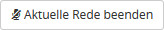
\includegraphics[scale=0.7]{clipart/Aktuelle-Rede-beenden}.
Gibt es mehrere Redner, kann man mit Klicken auf \includegraphics[scale=0.7]{clipart/N�chste-Rede-beginnen}
die aktuelle Rede beenden und die n�chste beginnen.

In der Rubrik \textsf{Letzte Redner/innen} k�nnen sie sich die letzten
Redner als Liste anzeigen lassen. Ein Teil dieser Liste wird auch
projiziert, je nach den Einstellungen. F�r Details dazu siehe \ref{subsec:Einstellungen-Tagesordnung}.

Jede Redeliste ist erst einmal offen. Das hei�t, dass sich jeder angemeldete
Teilnehmer auf die Redeliste setzen kann. Um die Redeliste zu schlie�en,
damit das nicht mehr m�glich ist, klicken Sie auf den Knopf \includegraphics[scale=0.7]{clipart/Redeliste-schlie�en}.
Der Knopf �ndert sich nun zu \includegraphics[scale=0.7]{clipart/Redeliste-�ffnen}
und der neue Zustand wird im Projektor rot angezeigt:

\begin{center}

\includegraphics[scale=0.7]{clipart/Redeliste-ist-geschlossen}
\par\end{center}

Wie man die Redeliste modifiziert und einen Countdown mit einer Rede
verkn�pft ist in \ref{subsec:Rednerliste-verwalten} erkl�rt.

Weitere Details zur Tagesordnung finden Sie in \ref{sec:Tagesordnung}.

\newpage{}

\section{Teilnehmer verwalten}

In diesem Teil lernen Sie, wie Sie die Teilnehmer Ihrer Veranstaltungen
im System erfassen. Im Pr�sentationsmodus brauchen Sie grunds�tzlich
nur diejenigen Teilnehmer erfassen, die das System verwalten, Antr�ge
stellen oder unterst�tzen, auf Redelisten stehen oder bei Wahlen kandidieren.

\subsection{Anlegen eines Teilnehmers\label{subsec:Anlegen-eines-Teilnehmers}}

Sie k�nnen die Teilnehmer einzeln eintragen oder, wie in \ref{sec:Teilnehmer}
beschrieben, importieren. Eingetragenen Personen, die das System verwalten
sollen, m�ssen die entsprechenden Berechtigungen zugewiesen werden.

Zum Anlegen eines neuen Teilnehmers wechseln Sie zum Men� \textsf{Teilnehmende}
und klicken Sie oben rechts auf 
\includegraphics[scale=0.7]{clipart/Neu-Teilnehmer-Symbol}.
Geben Sie als Beispiel diesen neuen Teilnehmer ein:

\begin{center}
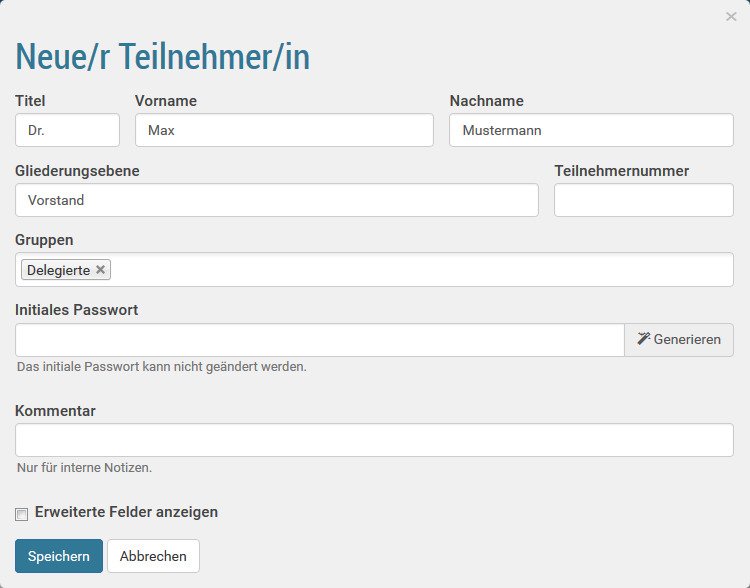
\includegraphics[width=1\columnwidth]{clipart/Teilnehmer-anlegen}
\par\end{center}

Wiederholen Sie diese Schritte und geben Sie folgende weitere Teilnehmer
und Teilnehmerinnen ein: Peter M�ller, Prof. Dr. Franziska Meyer,
Luise Schmidt und Dr. Hans Schulze.

Die Angabe des \textsf{Titels} und der \textsf{Gliederungsebene} ist
optional. �ber die \textsf{Gruppe} wird festgelegt, welche Berechtigungen
der Teilnehmer hat, also ob er z.\,B. w�hlen und Antr�ge stellen
darf. Mehr zu Gruppen ist in \ref{subsec:Gruppen} beschrieben.

\subsection{Bearbeiten eines Teilnehmers}

Im Men� \textsf{Teilnehmende} ist eine Liste mit allen Teilnehmern
zu sehen:

\begin{center}
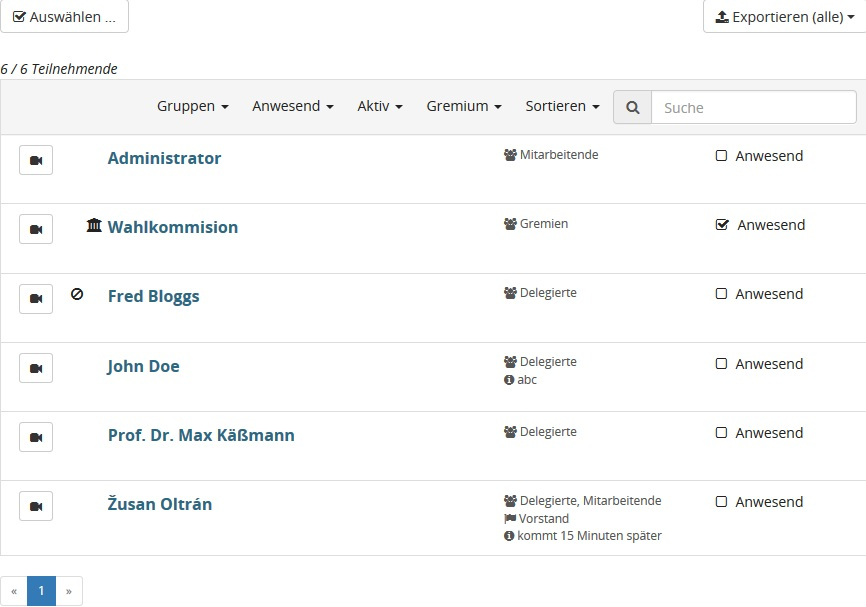
\includegraphics[width=1\columnwidth]{clipart/Teilnehmerliste}
\par\end{center}

Klicken Sie zum Bearbeiten beispielsweise beim Teilnehmer \quotedblbase Max~Mustermann\textquotedblleft{}
unterhalb des Namens auf \textsf{Bearbeiten} und weisen ihm zus�tzlich
die Gruppe \textsf{Mitarbeitende} zu.

In der Teilnehmerliste kann jederzeit eingestellt werden, ob ein Teilnehmer
anwesend ist. Dies ist f�r Wahlen und die Dokumentation der Veranstaltung
wichtig.

\subsection{Passwort eines Teilnehmers}

Beim Anlegen eines Teilnehmers wird automatisch ein zuf�lliges Erst-Passwort
gesetzt, falls man nicht selbst ein Passwort angibt. Sie k�nnen das
Erst-Passwort der PDF-Datei entnehmen, die durch Klick auf das Symbol

\includegraphics[scale=0.7]{clipart/PDF-Teilnehmer} und dann auf
\textsf{Zugangsdatenliste} angezeigt wird. Dieses PDF ist so ausgelegt,
dass man es ausdrucken und so jedem Teilnehmer seine Zugangsdaten
mitteilen kann.

Bitten Sie jeden, dem Sie sein Erst-Passwort aush�ndigen, dieses nach
dem ersten Login zu �ndern.

Um als Administrator das Passwort von zum Beispiel Max Mustermann
neu zu setzen, klicken Sie in der Teilnehmerliste unterhalb des Namens
auf \textsf{Bearbeiten} und tragen Sie im Feld \textsf{Voreingestelltes
Passwort} ein neues Passwort ein. Anschlie�end klicken Sie auf \textsf{Reset}
und dann erst auf \textsf{Speichern}.

Detaillierte, weitere Informationen zur Teilnehmerverwaltung finden
Sie in \ref{sec:Teilnehmer}.

\newpage{}

\section{Countdowns und Mitteilungen\label{sec:Countdowns-und-Mitteilungen}}

Unterhalb der Live-Vorschau gibt es die Rubriken \textsf{Countdown}
und \textsf{Mitteilungen}. Um z.\,B. mitzuteilen, wo es das Mittagessen
gibt, klicken Sie auf 
\includegraphics[scale=0.7]{clipart/Neue-Mitteilung}
und rechts oben in der Mitteilung auf 
\includegraphics[scale=0.7]{clipart/Bearbeiten-Symbol}.
Geben Sie nun den Text ,,Das Mittagessen gibt es in 5 Minuten im
Foyer, 1.~Stock, Aufgang B.`` ein und klicken anschlie�end auf 
\includegraphics[scale=0.7]{clipart/Haken-Symbol}.
Klicken Sie nun auf 
\includegraphics[scale=0.7]{clipart/Projektorsymbol},
wird die Mitteilung so angezeigt:

\begin{center}
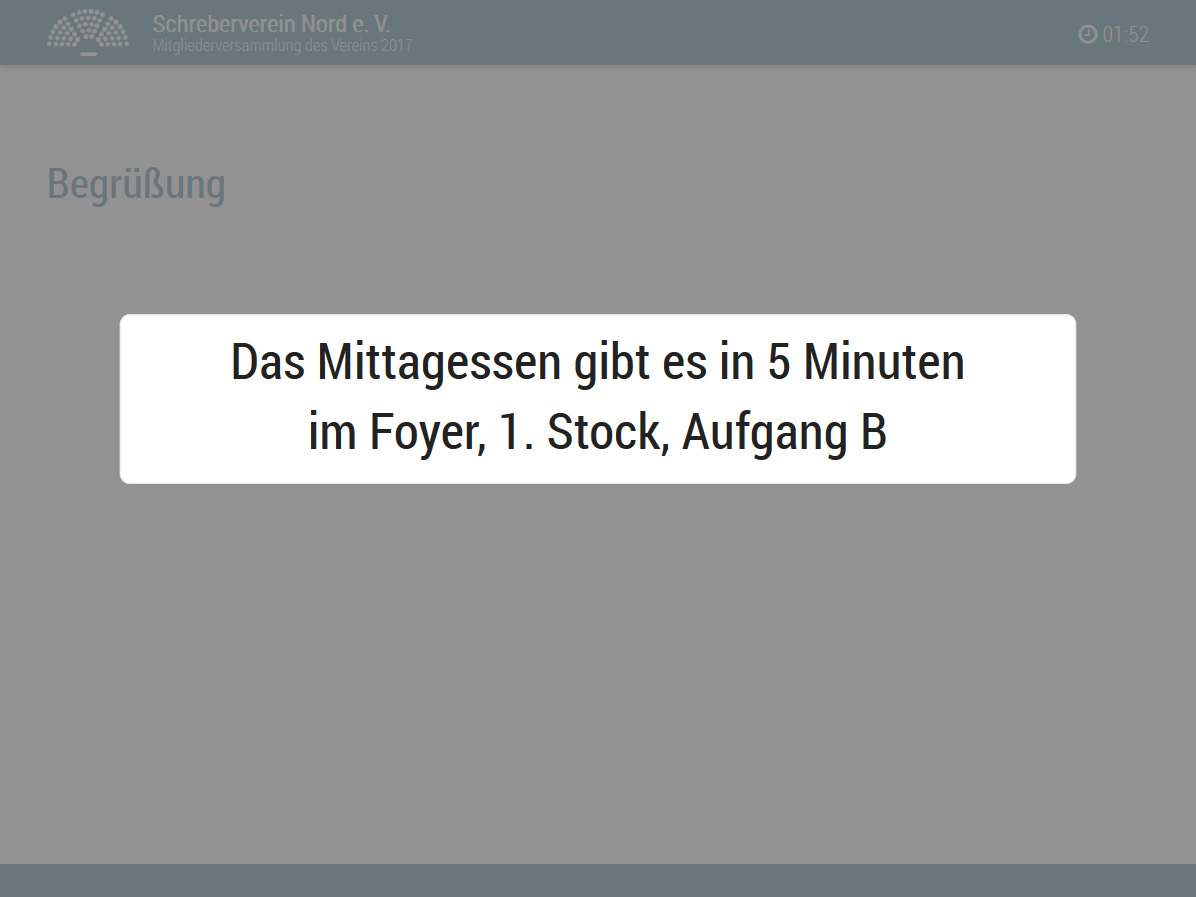
\includegraphics[width=1\columnwidth]{clipart/Mitteilung-Essen}
\par\end{center}

Um nun die 5\,min als Countdown laufen zu lassen, klicken Sie auf\\

\includegraphics[scale=0.7]{clipart/Neuer-Countdown} und dann auf

\includegraphics[scale=0.7]{clipart/Bearbeiten-Symbol}. Geben Sie
als \textsf{Beschreibung} ,,Mittagessen startet in`` und als \textsf{Startzeit}
,,5:00`` ein und klicken anschlie�end auf das Symbol 
\includegraphics[scale=0.7]{clipart/Haken-Symbol}.
Klicken Sie nun auf 
\includegraphics[scale=0.7]{clipart/Projektorsymbol}
um den Countdown anzuzeigen. Mit dem Klick auf 
\includegraphics[scale=0.7]{clipart/Projektorsymbol-laufend}
der aktuellen Mitteilung wird diese wieder von Projektor entfernt.
Klicken Sie auf 
\includegraphics[scale=0.7]{clipart/Countdown-Start-Symbol}
um den Countdown zu starten.

\begin{center}

\includegraphics[width=1\columnwidth]{clipart/Countdown-Beispiel}
\par\end{center}

Die Zeit des Countdowns wird unter 30\,s orange eingef�rbt. Nach
dem Ablauf wird die Zeit rot eingef�rbt und l�uft negativ.

Besonders sinnvoll sind Countdowns f�r Reden. Um f�r jede Rede einen
Countdown mitlaufen zu lassen, wechseln Sie in das Men� \textsf{Einstellungen\lyxarrow{}Tagesordnung}
und w�hlen dort die Option \textsf{Countdown mit der Redeliste verkoppeln}
aus. Nun werden alle Countdowns automatisch gestartet, wenn eine Rede
begonnen wird. Welchen Countdown Sie projizieren oder ob sie ihn �berhaupt
einen projizieren, haben Sie in der Hand.

\newpage{}

\section{Antr�ge verwalten und behandeln}

In diesem Teil lernen Sie, Antr�ge in das System einzugeben und zu
verwalten sowie, wie Sie w�hrend der Veranstaltung einen Antrag behandeln
und eine Abstimmung durchf�hren.

\subsection{Eingabe eines bereits vorliegenden Antrags}

Vor Beginn der Veranstaltung liegen bereits Antr�ge an die Versammlung
vor, welche ins System gebracht werden sollen. Wechseln Sie zum Men�
\textsf{Antr�ge} und klicken auf 
\includegraphics[scale=0.7]{clipart/Neu-Symbol}.

Geben Sie als Beispiel einen Antrag, mit dem die Vereinssatzung so
ge�ndert werden soll, dass der Beirat mehr Mitglieder hat, wie folgt
ein:

\newpage{}

\begin{center}
\includegraphics[width=1\columnwidth]{clipart/Antrag-ausf�llen}
\par\end{center}

Wie sie sehen, gibt es im Textfeld schon eine Einleitung ,,Die Versammlung
m�ge beschlie�en,``. Diese k�nnen Sie �ndern oder abschalten, siehe
dazu \ref{subsec:Einstellungen-Antr=0000E4ge}. Dass Sie den Antrag
als Tagesordnungspunkt anzeigen, ist optional.

Erstellen Sie auf gleiche Weise eine weiteren Antrag mit dem Titel
,,�nderung der Gesch�ftsordnung``.

Die Antragsseite sieht nun wie folgt aus:

\begin{center}
\includegraphics[width=1\columnwidth]{clipart/Antragsliste}
\par\end{center}

Antr�ge k�nnen auch w�hrend der Veranstaltung angelegt werden.

\subsection{Behandlung eines Antrags}

Angenommen die Versammlungsleitung ruft den Antrag zur Satzungs�nderung
auf. Klicken Sie zun�chst in der Antrags�bersicht auf \includegraphics[scale=0.7]{clipart/Projektorsymbol}
vor dem Antrag. Dieser wird nun projiziert:

\begin{center}
\includegraphics[width=1\columnwidth]{clipart/Antrag-projiziert}
\par\end{center}

Um schnell zur Antragsverwaltung zu wechseln, k�nnen Sie auf den Titel
des Antrags klicken.

Nach Abschluss der Diskussion ruft der Vorsitzende zur Abstimmung
auf. Klicken Sie im rechten Kasten auf \textsf{Neue Abstimmung} und
tragen Sie das Abstimmungsergebnis wie folgt in das Formular ein:

Der Vorsitzende stellt fest, dass der Antrag angenommen ist. Klicken
Sie deshalb auf der im rechten unteren Kasten unter \quotedblbase Antrag
verwalten\textquotedblleft{} auf \textsf{Annehmen}.

Das Projektorbild sieht nun wie folgt aus:

\newpage{}

\section{Wahlen durchf�hren}

In diesem Teil lernen Sie, wie Sie Wahlen auf Ihrer Versammlung mit
\noun{OpenSlides} begleiten.

\subsection{Anlegen von Wahlen}

Vor Veranstaltungsbeginn sind die anstehenden Wahlen vorzubereiten.
Gehen Sie dazu ins Men� \textsf{Wahlen}. Legen Sie nun eine neue Wahl
an indem sie oben auf \includegraphics[scale=0.7]{clipart/Neu-Symbol}
klicken. Geben Sie nun eine Wahl wie folgt ein:

\begin{center}
\includegraphics[width=1\columnwidth]{clipart/Wahl-eingeben}
\par\end{center}

Geben Sie auf die gleiche Weise eine weitere Wahl ein: 
\begin{description}
\item [{Name:}] Beirat
\item [{Beschreibung:}] Der Beirat unterst�tzt den Vorstand.
\item [{Anzahl~der~zur~Wahl~stehenden~Posten:}] 7
\end{description}
Die Wahl�bersicht sieht nun so aus:

\begin{center}
\includegraphics[width=1\columnwidth]{clipart/Wahl�bersicht}
\par\end{center}

\subsection{Durchf�hrung einer Wahl}

Klicken Sie in der Wahl�bersicht auf \includegraphics[scale=0.7]{clipart/Projektorsymbol}
vor \textsf{Vorstand}. Die Wahl wird nun projiziert. Nun klicken Sie
auf den Namen der Wahl \textsf{Vorstand}.

Setzen Sie sich mit \includegraphics[scale=0.7]{clipart/Redeliste+Mich}
auf die Kandidatenliste. Es k�nnen alle bei \noun{OpenSlides} angelegten
Teilnehmer hinzugef�gt werden. W�hlen Sie nun aus der Liste 4~weitere
Kandidaten aus.

Wir gehen nun davon aus, dass die Kandidatenliste feststeht. Damit
sich die Kandidaten vorstellen k�nnen, klicken Sie oben auf \includegraphics[scale=0.7]{clipart/Redeliste-Symbol}.
Die Redeliste ist technisch identisch zu der Redeliste eines Tagesordnungspunkts,
die in \ref{subsec:Redelisten} behandelt wurde. Wie Sie sehen, sind
bereits alle Kandidaten auf der Redeliste. Sie k�nnen noch weitere
Redner hinzuf�gen.

Um die Wahl zu beginnen, klicken Sie unten auf \includegraphics[scale=0.7]{clipart/Neuer-Wahlgang}.
Dadurch hat sich die Phase der Wahl automatisch auf \textsf{Im Wahlvorgang}
ge�ndert. Das Projektorbild sieht nun so aus:

\begin{center}
\includegraphics[width=1\columnwidth]{clipart/Wahl-Projektor}
\par\end{center}

Da die Wahl von Personen eine geheime Wahl ist, m�ssen Stimmzettel
erstellt werden. Klicken Sie daf�r auf \includegraphics[scale=0.7]{clipart/Stimmzettel-drucken}.
Der Stimmzettel sieht so aus:

\begin{center}
\includegraphics[scale=0.95]{clipart/Wahlzettel}
\par\end{center}

und kann ausgedruckt und verteilt werden.

Wir nehmen nun an, dass die Wahl ausgez�hlt wurde und die Ergebnisse
vorliegen. Tragen Sie daher nun die Ergebnisse dieses 1.\ Wahlgangs
ein, indem Sie auf \includegraphics[scale=0.7]{clipart/Stimmen-eingeben}
klicken. In die Eingabemaske tragen Sie als Beispiel bei Administrator
23, bei Frau Meyer 38, bei Herrn Mustermann 17, bei Herrn M�ller 20,
bei Frau Schmidt 22, bei \textsf{G�ltige Stimmen} 109, bei \textsf{Ung�ltige
Stimmen} 1 und bei \textsf{Abgegebene Stimmen} 110 ein.

Wir nehmen an, dass 50~Personen an der Wahl teilgenommen haben und
dass die Satzung vorsieht, dass die Personen gew�hlt sind, die mindestens
die H�lfte der Stimmen bekommen hat, wie Personen an der Wahl teilgenommen
haben. Es wurde also im 1.\ Wahlgang nur Frau Meyer gew�hlt. Klicken
Sie daher nur bei ihr auf das Symbol \includegraphics[scale=0.7]{clipart/Gew�hlt-Symbol}
vor ihrem Namen. Um die Wahl zu ver�ffentlichen, klicken Sie auf \includegraphics[scale=0.7]{clipart/Wahl-ver�ffentlichen}.
Im Projektor wird erst einmal nur die Kandidatenliste angezeigt, in
der Frau Meyer als Gew�hlte mit einem Stern markiert ist:

\begin{center}
\includegraphics[width=1\columnwidth]{clipart/Wahl-Projektor-Ergebnis}
\par\end{center}

Sie k�nnen nun entscheiden, ob auch die Stimmenanzahl ver�ffentlicht
wird. Da das gew�nscht ist, klicken Sie nun auf \includegraphics[scale=0.7]{clipart/Wahl-projizieren}.
Es wird nun dies projiziert:

\begin{center}
\includegraphics[width=1\columnwidth]{clipart/Wahl-Projektor-Ergebnis-Detail}
\par\end{center}

Als Erkl�rung k�nnen Sie nun vielleicht eine Mitteilung mit dem Inhalt
,,Es haben 50 Personen teilgenommen, zur Wahl notwendig waren daher
25 Stimmen.`` anzeigen, wie Sie es in \ref{sec:Countdowns-und-Mitteilungen}
gelernt haben.

Da der Vorstand aus 3~Personen bestehen muss, ist ein zweiter Wahlgang
notwendig. Klicken Sie daher auf \includegraphics[scale=0.7]{clipart/Neuer-Wahlgang}
und \includegraphics[scale=0.7]{clipart/Stimmzettel-drucken}. Geben
Sie fiktive Ergebnisse ein und markieren Herrn Mustermann und Administrator
als gew�hlt. Zuletzt klicken Sie auf \includegraphics[scale=0.7]{clipart/Wahl-ver�ffentlichen}
und \includegraphics[scale=0.7]{clipart/Wahl-projizieren} und �ndern
oben die Phase auf \textsf{Abgeschlossen}. Wenn Sie oben auf \includegraphics[scale=0.7]{clipart/PDF-Symbol}
klicken, erhalten Sie ein PDF mit dem Wahlergebnis, das Sie f�r die
Nachbereitung der Veranstaltung verwenden k�nnen.

Auf die gleiche Weise k�nnen Sie nun auch die die Wahl des Beirats
durchf�hren. Sie werden feststellen, dass als Wahlmethode automatisch
eine Ja-Nein-Enthaltungs-Wahl bez�glich eines jeden Kandidaten ausgew�hlt
wird, wenn es weniger oder gleich viele Kandidaten wie Pl�tze gibt:

\begin{center}
\includegraphics[scale=0.95]{clipart/Wahlzettel-Enthaltung}
\par\end{center}

Mehr zu Wahlen und deren Einstellungen erfahren Sie im Detail in \ref{subsec:Einstellungen-Wahlen}.

\newpage{}

\section{Dateien hochladen und verwalten}

Wie man Dateien, zum Beispiel Bilder, bei \noun{OpenSlides} hochl�dt
und projiziert, ist in \ref{sec:Dateien} erkl�rt.

\section{Nach einer Veranstaltung}

Am Ende der Versammlung k�nnen Sie sich f�r das Protokoll einige Dokumente
direkt aus \noun{OpenSlides} holen. Klicken Sie jeweils im Men� \textsf{Tagesordnung},
\textsf{Antr�ge}, \textsf{Wahlen} und \textsf{Teilnehmende} rechts
oben auf \includegraphics[scale=0.7]{clipart/PDF-Symbol}. Mehr zur
Nachbereitung ist in \ref{sec:Nachbereitung} beschrieben.

Alle weiteren Funktionen von \noun{OpenSlides} und Details zu den
im Tutorium behandelten Funktionen, finden Sie in \ref{chap:Einzelne-Funktionen}.
Wie Sie Anpassungen an \noun{OpenSlides} vornehmen, erfahren Sie
in \ref{chap:Weitere-Anpassungen-von}.

Viel Spa� weiterhin mit \noun{OpenSlides}!
\end{document}


%% LyX 2.2.0 created this file.  For more info, see http://www.lyx.org/.
%% Do not edit unless you really know what you are doing.
\documentclass[12pt,a4paper,ngerman,bibliography=totoc,index=totoc,BCOR7.5mm,titlepage,captions=tableheading,dvipsnames,table]{scrbook}
\usepackage{lmodern}
\renewcommand{\sfdefault}{lmss}
\renewcommand{\ttdefault}{lmtt}
\usepackage[T1]{fontenc}
\usepackage[latin9]{inputenc}
\setcounter{secnumdepth}{3}
\setlength{\parskip}{\medskipamount}
\setlength{\parindent}{0pt}
\usepackage{color}
\definecolor{note_fontcolor}{rgb}{0, 0, 1}
\usepackage{babel}
\usepackage{array}
\usepackage{float}
\usepackage{textcomp}
\usepackage{amsmath}
\usepackage{amssymb}
\usepackage{graphicx}
\usepackage[unicode=true,
 bookmarks=true,bookmarksnumbered=true,bookmarksopen=true,bookmarksopenlevel=2,
 breaklinks=true,pdfborder={0 0 1},backref=false,colorlinks=true]
 {hyperref}
\hypersetup{pdftitle={OpenSlides Handbuch},
 pdfauthor={OpenSlides Team},
 pdfsubject={OpenSlides Handbuch, Funktionen},
 pdfkeywords={OpenSlides, Handbuch, Funktionen},
 linkcolor=black, citecolor=black, urlcolor=blue, filecolor=blue, pdfpagelayout=OneColumn, pdfnewwindow=true, pdfstartview=XYZ, plainpages=false}

\makeatletter

%%%%%%%%%%%%%%%%%%%%%%%%%%%%%% LyX specific LaTeX commands.
\pdfpageheight\paperheight
\pdfpagewidth\paperwidth

\newcommand{\noun}[1]{\textsc{#1}}
\DeclareRobustCommand*{\lyxarrow}{%
\@ifstar
{\leavevmode\,$\triangleleft$\,\allowbreak}
{\leavevmode\,$\triangleright$\,\allowbreak}}
%% Because html converters don't know tabularnewline
\providecommand{\tabularnewline}{\\}
%% The greyedout annotation environment
\newenvironment{lyxgreyedout}
  {\textcolor{note_fontcolor}\bgroup\ignorespaces}
  {\ignorespacesafterend\egroup}

%%%%%%%%%%%%%%%%%%%%%%%%%%%%%% Textclass specific LaTeX commands.
\newcommand{\code}[1]{\texttt{#1}}

\@ifundefined{date}{}{\date{}}
%%%%%%%%%%%%%%%%%%%%%%%%%%%%%% User specified LaTeX commands.
% that links to image floats jumps
% to the beginning of the float and 
% not to its caption
\usepackage[figure]{hypcap}

% the pages of the TOC is numbered roman
% and a PDF-bookmark for the TOC is added
\let\myTOC\tableofcontents
\renewcommand\tableofcontents{%
  \frontmatter
  \pdfbookmark[1]{\contentsname}{}
  \myTOC
  \mainmatter }

% Linkfl�che f�r Querverweise vergr��ern und automatisch benennen,
\AtBeginDocument{\renewcommand{\ref}[1]{\mbox{\autoref{#1}}}}
\@ifpackageloaded{babel}{
 \addto\extrasngerman{%
  \renewcommand*{\equationautorefname}[1]{}%
  \renewcommand{\sectionautorefname}{Kap.\negthinspace}%
  \renewcommand{\subsectionautorefname}{Kap.\negthinspace}%
  \renewcommand{\subsubsectionautorefname}{Kap.\negthinspace}%
 }
}{}

% provides caption formatting
\usepackage[labelfont={bf,sf}]{caption}[2004/07/16]

% enables calculation of values,
\usepackage{calc}

% increase the bottom float placement fraction
\renewcommand{\bottomfraction}{0.5}

% avoids that floats are placed before their
% corresponding section starts
\let\mySection\section\renewcommand{\section}{\suppressfloats[t]\mySection}

% used to have extra space in table cells
\@ifundefined{extrarowheight}
 {\usepackage{array}}{}
\setlength{\extrarowheight}{2pt}

\makeatother

\begin{document}

\chapter{Einzelne Funktionen\label{chap:Einzelne-Funktionen}}

Im Folgenden werden die einzelnen Funktionen von \noun{OpenSlides}
erl�utert. Die Funktionen sind mit wenigen Ausnahmen alle �ber die
Men�punkte des Webinterfaces zu erreichen.

Die meisten der hier beschriebenen Funktionen sind nur f�r Administratoren
und Mitglieder der Teilnehmergruppe Mitarbeitende verf�gbar. Die Funktionen
f�r normale Mitglieder sind im Tutorium \emph{Teilnehmer} beschrieben,
siehe ??.

\section{An- und Abmelden \textendash{} Benutzername und Passwort �ndern\label{sec:An--und-Abmelden}}

\subsection{An- und Abmelden}

Beim ersten Aufruf von \noun{OpenSlides} erscheint die Login-Seite.

\begin{center}
\includegraphics[width=0.6666\columnwidth]{clipart/Login-Bildschirm}
\par\end{center}

Der erste Benutzername des Administrators ist \textsf{admin}. Er hat
das erste Passwort \textsf{admin}. �ber die Teilnehmerverwaltung\footnote{Mehr zur Teilnehmerverwaltung siehe \ref{sec:Teilnehmer}.}
neu angelegte Teilnehmer haben einen aus dem Vor- und Nachnamen zusammengesetzten
Benutzernamen, wobei Gro�- und Kleinschreibung zu beachten ist und
zwischen den Namen ein Leerzeichen liegt. Beispiel: Ein mit dem Vornamen
\textsf{Max} und dem Nachnamen \textsf{Mustermann} angelegter Teilnehmer
hat den Benutzernamen

\textsf{Max~Mustermann}

Das voreingestellte Passwort kann �ber die Teilnehmerverwaltung eingesehen
werden. Zum Einloggen geben Sie Ihren Benutzernamen und Ihr Passwort
ein und klicken auf \textsf{Anmelden}.

Um die Nutzer zu informieren wie man sich einloggt, kann man einen
Text im Men� \textsf{Einstellungen\lyxarrow{}Allgemein\lyxarrow{}System}
im Feld \textsf{Diesen Text auf der Login-Seite anzeigen} eingeben.
Dieser erscheint auf dem Login-Fenster, wenn sich die Teilnehmer einloggen:

\begin{center}
\includegraphics[width=0.6666\columnwidth]{clipart/Login-Bildschirm-angepasst}
\par\end{center}

\begin{lyxgreyedout}
\textbf{Hinweis:} \noun{OpenSlides} ben�tigt Cookies um die Identit�t
des Nutzers festzustellen, solange er eingeloggt ist. Beim Ausloggen
wird das Cookie wieder gel�scht.%
\end{lyxgreyedout}


\subsection{Eigenen Benutzernamen oder Passwort �ndern\label{subsec:Benutzername-oder-Passwort}}

Klickt man in der Kopfzeile von \noun{OpenSlides} rechts auf den
Benutzernamen, kann man das Profil bearbeiten oder das Passwort �ndern.

Die eigenen Benutzereinstellungen wie Benutzername und Passwort k�nnen
�ber den Button oben rechts ge�ndert werden. Klicken Sie auf den Button,
w�hlen Sie im oberen rechten Men� aus, ob Sie Ihre pers�nlichen Einstellungen
oder Ihr Passwort �ndern m�chten, und �ndern Sie die jeweiligen Einstellungen.
Klicken Sie abschlie�end auf \textsf{Speichern}.

\subsection{Fremde Benutzereinstellungen (insbesondere Benutzername oder Passwort)
�ndern}

Beim Anlegen eines Teilnehmers wird automatisch ein zuf�lliges Erst-Passwort
gesetzt. Sie k�nnen das voreingestellte Passwort aus einer PDF-Datei
ablesen, die Sie durch Klick auf den Link \quotedblbase Zugangsdatenliste\textquotedblleft{}
im rechten oberen Men� erreichen.

Benutzer mit den entsprechenden Rechten wie Mitarbeiter k�nnen alle
Benutzer �ber den Men�punkt \quotedblbase Teilnehmer/innen\textquotedblleft{}
verwalten und dort auch den Benutzernamen �ndern und das Passwort
auf ein bestimmtes voreingestelltes Passwort zur�cksetzen.

Klicken Sie beim jeweiligen Teilnehmer auf das Bearbeiten-Symbol \includegraphics[scale=0.67]{clipart/Bearbeiten-Symbol}
und tragen Sie unter \quotedblbase Voreingestelltes Passwort\textquotedblleft{}
ein neues, selbstgew�hltes Passwort ein. Anschlie�end klicken Sie
auf \textsf{�bernehmen}. In einem zweiten Schritt m�ssen Sie auf den
Link \quotedblbase Auf Erst-Passwort zur�cksetzen\textquotedblleft{}
klicken, um das im System gespeicherte Passwort mit Ihrem neu eingegebenen
zu ersetzen. Best�tigen Sie den oben auf der Seite erscheinenden Dialog
mit \textsf{Ja}.

\section{Projektorsteuerung}

Dieses Handbuch ist noch nicht fertiggestellt. Wenn Sie Interesse
haben, uns zu unterst�tzen, schreiben Sie uns einfach eine E-Mail:

\href{mailto:users-de@openslides.org}{users-de@openslides.org}

\newpage{}

\section{Countdown und Mitteilungen\label{sec:Countdown-und-Mitteilungen}}

Unterhalb der Live-Vorschau gibt es die Rubriken \textsf{Countdown}
und \textsf{Mitteilungen}.

\subsection{Countdowns\label{subsec:Countdowns}}

Um einen Countdown laufen zu lassen, klicken Sie auf \includegraphics[scale=0.7]{clipart/Neuer-Countdown}
und dann auf \includegraphics[scale=0.7]{clipart/Bearbeiten-Symbol}.
Geben Sie als \textsf{Beschreibung} einen kurzen Text ein, der sp�ter
unter der Zeit erscheint. Als \textsf{Startzeit} geben Sie eine Zeit
im Format \textsf{mm:ss} (Minuten:Sekunden, z.\,B: ,,5:00``) ein
und klicken anschlie�end auf \includegraphics[scale=0.7]{clipart/Haken-Symbol}.
Mit Klick auf \includegraphics[scale=0.7]{clipart/Projektorsymbol}
wird der Countdown angezeigt.

\begin{center}
\includegraphics[width=1\columnwidth]{clipart/Countdown-Beispiel}
\par\end{center}

Es ist m�glich mehrere Countdowns gleichzeitig zu projizieren. Die
Voreinstellung von 60\,s f�r die L�nge neuer Countdowns kann im Men�
\textsf{Einstellungen\lyxarrow{}Projektor} ge�ndert werden, siehe
\ref{subsec:Projektor}. Die Zeit der Countdowns wird unter 30\,s
orange eingef�rbt. Diese Zeit kann im Men� \textsf{Einstellungen\lyxarrow{}Tagesordnung}
ge�ndert werden, siehe \ref{subsec:Einstellungen-Tagesordnung}. Nach
dem Ablauf wird die Zeit rot eingef�rbt und l�uft negativ.

Um f�r jede Rede einen Countdown mitlaufen zu lassen, muss im Men�
\textsf{Einstellungen\lyxarrow{}Tagesordnung} die Option \textsf{Countdown
mit der Redeliste verkoppeln} ausgew�hlt sein. Dadurch werden alle
existierenden Countdowns automatisch gestartet, wenn eine Rede begonnen
wird. Ob, welcher und wie viele Countdowns projiziert werden, kann
durch das Klicken auf \includegraphics[scale=0.7]{clipart/Projektorsymbol}
festgelegt werden.

\subsection{Mitteilungen}

Um etwas mitzuteilen, klicken Sie auf \includegraphics[scale=0.7]{clipart/Neue-Mitteilung}
und rechts oben in der Mitteilung auf \includegraphics[scale=0.7]{clipart/Bearbeiten-Symbol}.
Geben Sie nun einen Text ein und klicken anschlie�end auf das Symbol
\includegraphics[scale=0.7]{clipart/Haken-Symbol}. Klicken Sie auf
\includegraphics[scale=0.7]{clipart/Projektorsymbol}, wird die Mitteilung
projiziert. Es kann immer nur eine Mitteilung projiziert werden.

\begin{center}
\includegraphics[width=1\columnwidth]{clipart/Mitteilung-Essen}
\par\end{center}

\newpage{}

\section{Tagesordnung\label{sec:Tagesordnung}}

Die Verwaltung der Tagesordnung ist im Men� \textsf{Tagesordnung}
angelegt. Dort wird die Tagesordnung in einer editierbaren Liste angezeigt.

\subsection{Tagesordnungspunkte erstellen und bearbeiten}

Um einen neuen Tagesordnungspunkt zu erstellen, klickt man oben rechts
auf \includegraphics[scale=0.7]{clipart/Neu-Symbol}. Der Text der
Tagesordnung kann frei formatiert werden und er kann auch Bilder und
Weblinks enthalten. Im Feld \textsf{Anhang} k�nnen Sie aus allen in
\noun{OpenSlides} verf�gbaren Dateien einen Anhang w�hlen. Mehr zu
Dateien siehe \ref{sec:Dateien}. Die Anh�nge werden nicht mit projiziert,
sie dienen nur f�r zus�tzliche Informationen.

Der Inhalt von Tagesordnungspunkten kann jederzeit ge�ndert werden,
insbesondere w�hrend der Veranstaltung. Dazu zeigt man mit der Maus
auf einen Tagesordnungspunkt und es erscheint ein Kontextmen�:

\begin{center}
\includegraphics[scale=0.95]{clipart/TOP-mit-Men�}
\par\end{center}

Klickt man dort auf \textsf{Bearbeiten}, kann man den Tagesordnungspunkt
bearbeiten. Als Alternative f�r das Bearbeiten kann man im Kontextmen�
auf \textsf{Quick-Edit} klicken und so oft ben�tigte Dinge wie die
\textsf{Dauer} �ndern:

\begin{center}
\includegraphics[width=1\columnwidth]{clipart/TOP-QuickEdit}
\par\end{center}

\textsf{Kommentare} dienen nur als Hinweis und werden nicht projiziert.
Sie sind nur f�r die Versammlungsleitung sichtbar.

\subsection{Einrichtung eigener Folien\label{subsec:Einrichtung-eigener-Folien}}

Eigene Folien werden verwendet, um Dinge au�erhalb der offiziellen
Tagesordnung zu behandeln. Technisch sind sie jedoch dasselbe wie
ein Tagesordnungspunkt. Das Erstellen einer eigenen Folie funktioniert
daher genauso wie das Erstellen eines Tagesordnungspunkts, nur dass
es wichtig ist, dass die Option \textsf{Als Tagesordnungspunkt anzeigen}
\emph{nicht} ausgew�hlt ist.

Eigene Folien werden in der �bersicht rosa unterlegt, um anzuzeigen,
dass sie nicht Teil der offiziellen Tagesordnung sind.

\subsection{Tagesordnungspunkte sortieren und nummerieren}

Die Tagesordnungspunkte werden entsprechend der aktuellen Sortierung
mit dem Knopf \includegraphics[scale=0.7]{clipart/Tagesordnung-nummerieren}
nummeriert. Die Art der Nummerierung kann �ber die Einstellungen festgelegt
werden, siehe \ref{subsec:Einstellungen-Tagesordnung}. So sieht eine
Tagesordnung aus, bei der r�mische Nummerierung und der Pr�fix ,,TOP``
gew�hlt wurde:

\begin{center}
\includegraphics[width=1\columnwidth]{clipart/Tagesordnung-speziell-nummeriert}
\par\end{center}

Die Reihenfolge der Tagesordnungspunkte kann jederzeit ver�ndert werden
und man kann Tagesordnungspunkte zu Unterpunkten machen. Dazu klickt
man oben auf den Knopf \includegraphics[scale=0.7]{clipart/Tagesordnung-sortieren}
und zieht mit gedr�ckter linker Maustaste einen Punkt an die gew�nschte
Stelle. Um aus einem Punkt einen Unterpunkt zu machen, schiebt man
ihn etwas nach rechts, bis er einrastet. Um einen Unterpunkt zu einem
Hauptpunkt zu machen, schiebt man ihn nach links. Nach der �nderung
der Reihenfolge muss man \includegraphics[scale=0.7]{clipart/Tagesordnung-nummerieren}
dr�cken, um die Nummerierung zu aktualisieren.

\subsection{Projektion der Tagesordnung}

Die komplette Tagesordnung wird projiziert, wenn man auf das Symbol\\
\includegraphics[scale=0.7]{clipart/Tagesordnung-projizieren} klickt.
Durch Dr�cken von \includegraphics[scale=0.7]{clipart/Untermen�-Symbol}
neben dem Symbol, kann man w�hlen, ob alle Tagesordnungspunkte oder
nur die Hauptpunkte angezeigt werden. Eigene Folie werden in der Tagesordnung
nicht projiziert.

Einzelne Tagesordnungspunkte werden projiziert, indem man auf das
Symbol \includegraphics[scale=0.7]{clipart/Projektorsymbol} vor dem
entsprechenden Eintrag klickt. So k�nnen eigene Folien projiziert
werden.

\subsection{Redeliste verwalten\label{subsec:Rednerliste-verwalten}}

\noun{OpenSlides} verf�gt bei jedem Tagesordnungseintrag �ber eine
Redelistenfunktion. Um eine Redeliste zu erstellen oder zu bearbeiten,
klickt man im Kontextmen� des jeweiligen Tagesordnungspunkts auf \textsf{Redeliste}.
Alternativ klickt man auf den Tagesordnungspunkt und dann auf \includegraphics[scale=0.7]{clipart/Redeliste-Symbol}.

Mit einem Klick auf \includegraphics[scale=0.7]{clipart/Redeliste+Mich}
kann man sich selbst auf die Redeliste setzen. Administratoren k�nnen
jeden auf die Redeliste setzen und durch Klicken von \includegraphics[scale=0.7]{clipart/Redner-entfernen}
jeden von der Liste nehmen.

Die Redeliste wird durch Klicken auf \includegraphics[scale=0.7]{clipart/Projektorsymbol-Redeliste}
projiziert. Durch Dr�cken von \includegraphics[scale=0.7]{clipart/Rede-beginnen}
wird eine Rede gestartet. Der Name des Redners wird nun im Projektor
angezeigt.

Um f�r jede Rede einen Countdown mitlaufen zu lassen, muss in den
Einstellungen, siehe \ref{subsec:Einstellungen-Tagesordnung}, die
Option \textsf{Countdown mit der Redeliste verkoppeln} ausgew�hlt
sein. Dadurch werden alle existierenden Countdowns automatisch gestartet,
wenn eine Rede begonnen wird. Ob, welcher und wie viele Countdowns
projiziert werden, kann durch das Klicken auf \includegraphics[scale=0.7]{clipart/Projektorsymbol}
vor den Countdowns festgelegt werden. Mehr zu Countdowns ist in \ref{subsec:Countdowns}
beschrieben.

Um die Rede zu beenden, klickt man auf \includegraphics[scale=0.7]{clipart/Aktuelle-Rede-beenden}
oder \includegraphics[scale=0.7]{clipart/Rede-beenden}. Gibt es mehrere
Redner, kann man mit Klicken auf \includegraphics[scale=0.7]{clipart/N�chste-Rede-beginnen}
die aktuelle Rede beenden und die n�chste beginnen.

In der Rubrik \textsf{Letzte Redner/innen} kann man sich die letzten
Redner als Liste anzeigen lassen. Die letzten x~Redner dieser Liste
werden auch projiziert. Die Anzahl der projizierten Redner kann eingestellt
werden, siehe \ref{subsec:Einstellungen-Tagesordnung}.

Jede Redeliste ist erst einmal offen. Das hei�t, dass sich jeder angemeldete
Teilnehmer auf die Redeliste setzen kann. Um die Redeliste zu schlie�en,
damit das nicht mehr m�glich ist, klickt man den Knopf \includegraphics[scale=0.7]{clipart/Redeliste-schlie�en}.
Der Knopf �ndert sich nun zu \includegraphics[scale=0.7]{clipart/Redeliste-�ffnen}
und der neue Zustand wird im Projektor rot angezeigt.

Die Reihenfolge der Redeliste kann jederzeit ge�ndert werden. Dazu
klickt man auf das Symbol \includegraphics[scale=0.7]{clipart/Redner-verschieben}
vor dem Rednernamen, h�lt die Maustaste gedr�ckt und verschiebt den
Redner an die gew�nschte Stelle.

Am Ende der Veranstaltung kann man s�mtliche Redelisten mit den jeweiligen
Redezeiten als CSV-Datei exportieren. Dazu ben�tigt man das Plugin
\emph{CSV Export Plugin for OpenSlides}, das in \ref{subsec:Das-Plugin-CSV}
beschrieben ist.

\subsection{Tagesordnung drucken\label{subsec:Tagesordnung-drucken}}

Auf der �bersichtsseite der Tagesordnung kann man durch Klicken auf
\includegraphics[scale=0.7]{clipart/PDF-Symbol} die gesamte Tagesordnung
mit allen Unterpunkten (ohne eigene Folien) als PDF-Datei abrufen.

\subsection{Einstellungen\label{subsec:Einstellungen-Tagesordnung}}

Im Men�punkt \textsf{Einstellungen\lyxarrow{}Tagesordnung} kann das
Verhalten der Tagesordnung konfiguriert werden.

\subsubsection*{Rubrik Allgemein}

Im Feld \textsf{Pr�fix f�r Nummerierung von Tagesordnungspunkten}
kann man einen Pr�fix angeben, der vor der Nummer des Tagesordnungspunkts
angezeigt wird; z.\,B. ,,TOP``.

Im Feld \textsf{Nummerierungssystem f�r Tagesordnungspunkte} kann
die Nummerierung der Tagesordnungspunkte zwischen arabischen und r�mischen
Nummern umgeschaltet werden.

Im Feld \textsf{Beginn der Veranstaltung} wird der genaue Beginn der
Veranstaltung angegeben. Das Eingabeformat ist dabei \textsf{TT.MM.JJJJ
HH:MM}; also z.\,B. ,,\textsf{02.03.2017~10:00}``.

\subsubsection*{Rubrik Redeliste}

Im Feld \textsf{Anzahl der dargestellten letzten Redner/innen auf
dem Projektor} kann die Anzahl der letzten Redner eingestellt werden,
die als Liste �ber der Liste der folgenden Redner angezeigt wird.
Im Projektor ist diese Liste in grauer Schrift:

\newpage{}

\begin{center}
\includegraphics[scale=0.7]{clipart/Redeliste-Projektor}
\par\end{center}

Im Feld \textsf{Countdown in den letzten x Sekunden der Redezeit orange
darstellen} kann man einstellen, die wie viele der letzten Sekunden
eines Countdowns in orange dargestellt werden.

Mit der Option \textsf{Countdown mit der Redeliste verkoppeln} werden
bei Beginn jeder Rede alle existierenden Countdowns gestartet. Mehr
zu Countdowns siehe \ref{subsec:Countdowns}.

\newpage{}

\section{Teilnehmer\label{sec:Teilnehmer}}

Die Teilnehmerverwaltung ist im Men� \textsf{Teilnehmende} angelegt.
Dort werden alle angelegten Teilnehmer in einer editierbaren Liste
angezeigt.

\subsection{Manuelles Anlegen}

Zum manuellen Anlegen eines neuen Teilnehmers klickt man oben rechts
auf \includegraphics[scale=0.7]{clipart/Neu-Teilnehmer-Symbol}. In
der erscheinenden Eingabemaske k�nnen folgende Angaben gemacht werden: 
\begin{description}
\item [{Benutzername}] Benutzername des Teilnehmers, mit dem er sich in
\noun{OpenSlides} einloggt.
\item [{Titel}] optionaler Titel des Teilnehmers. Dieser wird z.\,B. in
Redelisten vor dem Namen angezeigt
\item [{Vorname}] Vorname 
\item [{Nachname}] Nachname
\item [{Gliederungsebene}] optionale Angabe der Mitgliedschaft in einer
Organisation. Bei Veranstaltungen von Vereinen kann man so z.\,B.
f�r Vorstandsmitglieder ,,Vorstand`` eintragen. Die Gliederungsebene
wird z.\,B. in Redelisten nach dem Namen angezeigt
\item [{Gruppen}] Gruppe(n), der der Teilnehmer in \noun{OpenSlides} angeh�rt.
Man kann nacheinander mehrere Gruppen ausw�hlen. Mehr dazu siehe \ref{subsec:Gruppen}.
\item [{Voreingestelltes~Passwort}] Das Erst-Passwort f�r den Teilnehmer.
Wird keines angegeben, wird automatisch eins generiert, siehe \ref{subsec:Passwort-und-Zugangsdaten}.
\item [{Kommentar}] optionaler Kommentar zum Teilnehmer
\item [{�ber~mich}] optionale pers�nliche Informationen zum Teilnehmer
\item [{Ist~anwesend}] Anwesenheitsstatus, der sp�ter auch direkt in der
Teilnehmerliste gesetzt werden kann.
\item [{Ist~aktiv}] Option, die bestimmt, ob der Teilnehmer als aktiv
behandelt werden soll. Man kann ihn so deaktivieren, ohne ihn zu l�schen.
\end{description}
In der Praxis kann es sein, dass man oft nicht mehr angibt als den
Namen. Es ist daher auch m�glich Teilnehmer anzulegen, indem man oben
rechts auf \includegraphics[scale=0.7]{clipart/Importieren-Symbol}
klickt. Dort gibt man in das Textfeld nur den Vor- und Nachnamen ein.
Mit weiteren Zeilen im Textfeld k�nnen auch gleich mehrere Teilnehmer
angelegt werden. Abschlie�end klickt man auf \includegraphics[scale=0.7]{clipart/Importieren-Knopf}.
In der Teilnehmerliste, siehe \ref{subsec:Teilnehmerliste}, kann
man nachtr�glich weitere Informationen hinzuf�gen.

\subsection{Automatisiertes Anlegen}

Teilnehmer k�nnen automatisiert aus einer Liste importiert werden.
Dazu muss eine CSV-Datei erstellt werden. Dies ist eine Textdatei
(die �blicherweise die Endung \textsf{.csv} oder seltener \textsf{.txt}
hat). Ihre erste Zeile muss aus dieser Zeile bestehen:

\code{title,first\_name,last\_name,structure\_level,groups,comment,is\_active}

Es folgen dann je eine Zeile f�r jeden Teilnehmer. Ein Eintrag f�r
einen Teilnehmer w�re z.\,B.:

\code{Prof. Dr.,Max,K��mann,{,}3,{,}1}

Jedes Komma trennt die Eigenschaften voneinander. Gibt es eine Eigenschaft
nicht, folgen die Kommas direkt aufeinander. Es muss jedoch mindestens
der Vor- und Nachname angegeben werden. Bei der Anwesenheit bedeutet
'1', dass die Person anwesend ist oder sein wird, ansonsten verwendet
man '0' oder nichts.\\
Bei der Gruppe wird nicht deren Name, sondern deren Nummer angegeben.
Voreingestellt in \noun{OpenSlides} ist Gruppe~\textsf{3} f�r \emph{Delegierte}
und Gruppe~\textsf{4} f�r \emph{Mitarbeitende}; Details dazu siehe
\ref{subsec:Gruppen}. Soll ein Teilnehmer in mehreren Gruppen sein,
werden diese durch Komma getrennt in Anf�hrungszeichen gesetzt also
z.\,B.:

\code{,�usan,Oltr�n,Vorstand,\textquotedbl{}3,4\textquotedbl{},kommt 15
Minuten sp�ter,}

\begin{lyxgreyedout}
\textbf{Achtung:} Die Gruppen~1 und 2 werden von OpenSlides automatisch
vergeben. Man darf diese Gruppennummern in der der CSV-Datei nicht
vergeben, da der Teilnehmer sonst nicht angelegt wird.%
\end{lyxgreyedout}

Zum Importieren klickt man oben rechts auf \includegraphics[scale=0.7]{clipart/Importieren-Symbol}.
Dort stellt man in der Rubrik \textsf{Import von CSV-Datei} die \textsf{Kodierung}
auf UTF-8. Das stellt sicher, dass Namen mit Akzenten, Umlauten usw.\ korrekt
importiert werden. Dazu muss die CSV-Datei auch mit der Kodierung
UTF-8 gespeichert worden sein. (Daf�r reicht es bei den meisten Editor-Programmen
aus, dass man Unicode f�r die Kodierung einstellt, falls das nicht
schon automatisch die Voreinstellung ist.) Nun klickt man auf den
Knopf \textsf{Durchsuchen} und w�hlt eine CSV-Datei aus. Nach wenigen
Sekunden sieht man in der Vorschau was importiert werden wird:\footnote{Den Inhalt der CSV-Datei, die f�r dieses Bildschirmfoto verwendet
wurde, ist in \ref{chap:Beispiel-f=0000FCr-Teilnehmer} zu finden.}

\newpage{}

\begin{center}
\includegraphics[width=1\columnwidth]{clipart/Import-Teilnehmer-Vorschau}
\par\end{center}

und kann die CSV-Datei noch �ndern, falls es Fehler gibt. Zum Import
dr�ckt man auf den blauen Knopf \textsf{x~Teilnehmende~importieren}.

Der Benutzername, mit dem sich ein importierter Teilnehmer bei \noun{OpenSlides}
einloggt, ist immer \textsf{Vorname\textvisiblespace{}Nachnahme}
(z.\,B.\textsf{ �usan\textvisiblespace{}Oltr�n}). Gibt es mehrere
Personen mit exakt dem gleichen Namen, hat eine davon den Zusatz '\textvisiblespace{}1'
(z.\,B.\textsf{ �usan\textvisiblespace{}Oltr�n\textvisiblespace{}1}).

CSV-Dateien lassen sich �brigens recht einfach mit g�ngigen Tabellenkalkulationsprogrammen
wie \noun{\href{http://www.libreoffice.org/}{LibreOffice}} oder \noun{Excel}
erstellen. Dazu erstellt man einfach eine Tabelle in dieser Form:

\begin{center}
\begin{tabular}{|c|c|c|c|c|c|c|}
\hline 
title & first\_name & last\_name & structure\_level & groups & comment & is\_active\tabularnewline
\hline 
 & John & Doe &  & 4 & abc & 1\tabularnewline
\hline 
 &  &  &  &  &  & \tabularnewline
\hline 
\end{tabular}
\par\end{center}

und speichert sie als CSV-Datei mit der Kodierung \emph{UTF-8} und
dem Komma als Trennzeichen. Es k�nnen so bestehende Mitgliedslisten
f�r \noun{OpenSlides} aufbereitet werden.

\subsection{Teilnehmerliste\label{subsec:Teilnehmerliste}}

Alle Teilnehmer werden in der Teilnehmerliste aufgef�hrt. Die Liste
kann durchsucht werden und man kann sie so modifizieren, dass durch
Klicken auf \includegraphics[scale=0.7]{clipart/Teilnehmer-Filter-Symbol}
nur Teilnehmer bestimmter Gruppen oder nur anwesende Teilnehmer angezeigt
werden. Durch Klicken auf eine Spalten�berschrift wird die Liste entsprechend
sortiert. In der Spalte \textsf{Anwesend} kann jederzeit die Anwesenheit
eingestellt werden.

Durch das Klicken auf den Namen eines Teilnehmers, werden dessen Daten
angezeigt. Durch Klicken unterhalb des Namens kann man den Teilnehmer
bearbeiten oder l�schen. F�r das Bearbeiten erscheint dieselbe Eingabemaske
wie beim manuellen Anlegen.

Durch Klicken auf \includegraphics[scale=0.7]{clipart/Teilnehmer-Ausw�hlen-Symbol}
k�nnen mehrere Teilnehmer ausgew�hlt und f�r diese eine bestimmte
Operation durchgef�hrt werden.

Die Teilnehmerliste kann auch als PDF ausgedruckt werden, wenn man
auf das Symbol \includegraphics[scale=0.7]{clipart/PDF-Teilnehmer}
und dann auf \includegraphics{clipart/Teilnehmerliste-Export} klickt.

\subsection{Passwort und Zugangsdaten\label{subsec:Passwort-und-Zugangsdaten}}

Beim Anlegen eines Teilnehmers wird automatisch ein zuf�lliges Erst-Passwort
gesetzt, falls man nicht manuell ein Passwort angibt. Die Erst-Passw�rter
aller Teilnehmer sind in einer Datei hinterlegt, die durch Klick auf
das Symbol \includegraphics[scale=0.7]{clipart/PDF-Teilnehmer} und
dann auf \textsf{Zugangsdatenliste} angezeigt wird. Dieses PDF ist
so ausgelegt, dass man es ausdrucken und so jedem Teilnehmer seine
Zugangsdaten mitteilen kann. Der Inhalt des PDFs kann �ber die Teilnehmereinstellungen
ge�ndert werden, siehe \ref{subsec:Einstellungen-Benutzer}.

Das Erst-Passwort sollte von jedem Teilnehmer schnellstm�glich ge�ndert
werden.

Administratoren haben die M�glichkeit das Passwort jedes Teilnehmers
manuell neu zu setzen, indem sie die Benutzerdaten bearbeiten.

\begin{lyxgreyedout}
\textbf{Achtung:} Beim �ndern des Passworts muss es zuerst ge�ndert
werden und an schlie�end auf \textsf{Reset} gedr�ckt gerden. Das ist
wichtig, denn ansonsten wird das neue Passwort nicht in die Datenbank
eingetragen, obwohl es im PDF mit den Zugangsdaten auftaucht.%
\end{lyxgreyedout}


\subsection{Gruppen\label{subsec:Gruppen}}

�ber die Zugeh�rigkeit zu einer Gruppe wird festgelegt, was ein Teilnehmer
bei der Veranstaltung und in \noun{OpenSlides} darf. Klick man auf
\includegraphics[scale=0.7]{clipart/Gruppen-Symbol}, wird eine Liste
mit allen aktuell existierenden Gruppen angezeigt.

Klickt man auf den Namen einer Gruppe, werden deren Berechtigungen
angezeigt. Um die Gruppeneigenschaften zu �ndern, klickt man auf \includegraphics[scale=0.7]{clipart/Bearbeiten-Symbol}.
Die aktuellen Berechtigungen sind blau unterlegt. Um eine Berechtigung
hinzuzuf�gen, h�lt man die \textsf{Strg}-Taste gedr�ckt und klickt
dann auf die entsprechende Berechtigung. H�lt man die \textsf{Strg}-Taste
gedr�ckt und klickt auf eine bereits ausgew�hlte Berechtigung, wird
diese abgew�hlt.

\begin{lyxgreyedout}
\textbf{\textcolor{blue}{Achtung!}}\textcolor{blue}{: Beim �ndern
der Berechtigungen muss die }\textsf{\textcolor{blue}{Strg}}\textcolor{blue}{-Taste
immer gedr�ckt gehalten sein, da sonst alle anderen Berechtigungen
automatisch abgew�hlt werden.}\footnote{Dies ist \noun{OpenSlides} \href{https://github.com/OpenSlides/OpenSlides/issues/2120}{bug \#{}2120}.}
\ref{chap:Voreinstellungen-der-Teilnehmer-} listet die Voreinstellungen
der Gruppen auf.%
\end{lyxgreyedout}

Eine neue Gruppe kann durch Klicken auf \includegraphics[scale=0.7]{clipart/Neu-Symbol}
erstellt werden.

Die Gruppen \textsf{G�ste} und \textsf{Registrierte~Nutzer} werden
automatisch zugewiesen. Alle angemeldeten Teilnehmer geh�ren zur Gruppe
\textsf{Registrierte~Nutzer}, alle unangemeldeten und damit anonymen
Teilnehmer geh�ren zur Gruppe \textsf{G�ste}. 

Unangemeldete Teilnehmer k�nnen die Veranstaltung nur sehen, wenn
im Men� \textsf{Einstellungen\lyxarrow{}Allgemein\lyxarrow{}System}
die Option \textsf{Erlaube Zugriff f�r anonyme Gast-Nutzer} aktiviert
ist.

\subsection{Einstellungen\label{subsec:Einstellungen-Benutzer}}

Im Men� \textsf{Einstellungen\lyxarrow{}Benutzer} k�nnen Einstellungen
f�r die Benutzerverwaltung vorgenommen werden.

\subsubsection*{Rubrik Sortierung}

Mit der Option \textsf{Benutzer nach Vornamen sortieren }werden die
Teilnehmer in der Teilnehmerliste nach Vornamen statt nach Nachnamen
sortiert.

\subsubsection*{Rubrik PDF}

Im Feld \textsf{Titel f�r das Zugangsdaten- und Begr��ungs-PDF} wird
der Titel eingegeben, der im PDF der Zugangsdaten erscheint, das man
an die Teilnehmer austeilen kann. Mehr dazu siehe \ref{subsec:Passwort-und-Zugangsdaten}.

Im Feld \textsf{Hilfetext f�r das Zugangsdaten- und Willkommens-PDF}
wird der Text eingegeben, der im PDF der Zugangsdaten erscheint.

Im Feld \textsf{System URL} wird die URL angegeben, auf der sich die
Teilnehmer einloggen k�nnen. Dort l�uft der \noun{OpenSlides} Server.

Im Feld \textsf{WLAN-Name (SSID)} kann der Name eines WLANs angegeben
werden.

Im Feld \textsf{WLAN-Passwort} kann das Passwort f�r das WLAN angegeben
werden.

Im Feld \textsf{WLAN-Verschl�sselung} kann die Verschl�sselung des
WLANs angegeben werden.

Die Angaben f�r das WLAN und die \textsf{System URL} erscheinen im
PDF der Zugangsdaten und werden auch im QR-Code in diesem PDF ber�cksichtigt.

\newpage{}

\section{Antr�ge\label{sec:Antr=0000E4ge}}

\subsection{Manuelles Erstellen von Antr�gen\label{subsec:Manuelles-Erstellen-von}}

Um einen neuen Antrag zu erstellen, klickt man im Men� \textsf{Antr�ge}
oben auf \includegraphics[scale=0.7]{clipart/Neu-Symbol}. In der
erscheinenden Eingabemaske wird der Antragsteller, der Titel des Antrags,
der Antragstext und die Begr�ndung eingetragen.

Wird die Option \textsf{Als Tagesordnungspunkt anzeigen} ausgew�hlt,
erscheint die Wahl als Tagesordnungspunkt. Ansonsten erscheint die
Wahl in der Tagesordnungs�bersicht als eigene Folie. Siehe \ref{subsec:Einrichtung-eigener-Folien}
f�r mehr zu eigenen Folien. Mit der Option \textsf{Erweiterte Felder
anzeigen }kann au�erdem ein Sachgebiet,\footnote{Siehe \ref{subsec:Sachgebiete} f�r Infos zu Sachgebieten.}
Schlagw�rter,\footnote{Siehe \ref{subsec:Schlagw=0000F6rter } f�r Infos zu Schlagw�rtern.}
die Unterst�tzer und der Arbeitsablauf\,\footnote{Siehe \ref{subsec:Arbeitsablauf-und-Status} f�r Infos zu Arbeitsabl�ufen.}
angegeben werden.

Klickt man oben auf \includegraphics[scale=0.7]{clipart/PDF-Symbol},
wird ein PDF mit der �bersicht aller angelegten Antr�ge generiert.
Den Titel und Inhalt des PDFs kann man �ber die Einstellungen festlegen,
siehe \ref{subsec:Einstellungen-Antr=0000E4ge}. Es erscheint im PDF
zuerst die Liste aller Sachgebiete, dann die Liste der Antr�ge und
schlussendlich jeder Antrag komplett mit Begr�ndung. Die Antr�ge k�nnen
so auch ausgedruckt und verteilt werden.

\subsection{Automatisiertes Erstellen von Antr�gen}

Antr�ge k�nnen automatisiert aus einer Liste importiert werden. Dazu
muss eine CSV-Datei erstellt werden. Dies ist eine Textdatei (die
�blicherweise die Endung \textsf{.csv} oder seltener \textsf{.txt}
hat). Ihre erste Zeile muss aus dieser Zeile bestehen:

\code{identifier,title,text,reason,submitter,category}

Es folgen dann je eine Zeile f�r jeden Antrag. Ein Eintrag f�r einen
Antrag w�re z.\,B.:

\textsf{Kat A-1,Satzungs�nderung,\textquotedbl{}Die Mitgliederversammlung
m�ge beschlie�en, in �8 Absatz 1 der Vereinssatzung die Zahl f�nf
durch sieben zu ersetzen.\textquotedbl{},Die vielen Aufgaben erfordern
eine Erweiterung des Beirates auf sieben Mitglieder.,Dr. Hans Schulze,Kategorie
A}

Jedes Komma trennt die Eigenschaften voneinander. Gibt es eine Eigenschaft
nicht, folgen die Kommas direkt aufeinander. Es muss jedoch mindestens
der Titel und Text angegeben werden. Enth�lt eine Eigenschaft ein
Komma, muss die Eigenschaft in doppelte Anf�hrungszeichen gesetzt
werden. Dies wurde in obigem Beispiel f�r den Antragstext gemacht.
Beim Antragsteller ist es wichtig, dass er mit seinem Titel angegeben
wird. In obigem Beisiel ist der Benutzername bei \noun{OpenSlides}
zwar ,,Hans Schulze``, hier muss er aber als ,,Dr. Hans Schulze``
angegeben werden, wenn er mit diesem Titel in \noun{OpenSlides} angelegt
ist.

Zum Importieren klickt man oben rechts auf \includegraphics[scale=0.7]{clipart/Importieren-Symbol}.
Dort stellt man in der Rubrik \textsf{Import von CSV-Datei} die \textsf{Kodierung}
auf UTF-8. Das stellt sicher, dass Namen mit Akzenten, Umlauten usw.\ korrekt
importiert werden. Dazu muss die CSV-Datei auch mit der Kodierung
UTF-8 gespeichert worden sein. (Daf�r reicht es bei den meisten Editor-Programmen
aus, dass man Unicode f�r die Kodierung einstellt, falls das nicht
schon automatisch die Voreinstellung ist.) Nun klickt man auf den
Knopf \textsf{Durchsuchen} und w�hlt eine CSV-Datei aus. Nach wenigen
Sekunden sieht man in der Vorschau was importiert werden wird:\footnote{Den Inhalt der CSV-Datei, die f�r dieses Bildschirmfoto verwendet
wurde, ist in \ref{chap:Beispiel-f=0000FCr-Antrag} zu finden.}

\begin{center}
\includegraphics[width=1\columnwidth]{clipart/Import-Antr�ge-Vorschau}
\par\end{center}

und kann die CSV-Datei noch �ndern, falls es Fehler gibt. Wie man
sieht, werden noch nicht existierende Kategorien und Antragsteller
beim Importieren automatisch angelegt. Zum Import dr�ckt man auf den
blauen Knopf \textsf{x~Antr�ge~importieren}.

Gibt es bereits einen Antrag mit demselben Bezeichner, wird der Antrag
nicht importiert. Gibt es einen Antrag mit demselben Titel bereits,
wird dieser importiert, da der Antragsteller das nicht wissen kann.
Man muss diesem Antrag dann manuell einen geeigneten Titel geben.

CSV-Dateien lassen sich �brigens recht einfach mit g�ngigen Tabellenkalkulationsprogrammen
wie \noun{\href{http://www.libreoffice.org/}{LibreOffice}} oder \noun{Excel}
erstellen. Dazu erstellt man einfach eine Tabelle in dieser Form:

\begin{center}
\begin{tabular}{|>{\centering}p{0.1\columnwidth}|>{\centering}p{0.08\columnwidth}|>{\centering}p{0.22\columnwidth}|>{\centering}p{0.22\columnwidth}|>{\centering}p{0.11\columnwidth}|>{\centering}p{0.1\columnwidth}|}
\hline 
identifier & title & text & reason & submitter & category\tabularnewline
\hline 
Kat A-1 & Sat\-zungs\-�nde\-rung & Die Mitgliederversammlung m�ge beschlie�en, in �8 Absatz 1 der Vereinssatzung
die Zahl f�nf durch sieben zu ersetzen. & Die vielen Aufgaben erfordern eine Erweiterung des Beirates auf sieben
Mitglieder. & Dr. Hans Schulze & Kate\-gorie~A\tabularnewline
\hline 
 &  &  &  &  & \tabularnewline
\hline 
\end{tabular}
\par\end{center}

und speichert sie als CSV-Datei mit der Kodierung \emph{UTF-8} und
dem Komma als Trennzeichen. Es k�nnen so bestehende Mitgliedslisten
f�r \noun{OpenSlides} aufbereitet werden.

\subsection{Bearbeiten von Antr�gen}

Der Inhalt von Antr�gen kann jederzeit ge�ndert werden, insbesondere
w�hrend der Veranstaltung. Dazu zeigt man mit der Maus auf einen Antrag
und es erscheint ein Kontextmen�:

\begin{center}
\includegraphics[scale=0.95]{clipart/Antrag-mit-Men�}
\par\end{center}

Klickt man dort auf \textsf{Bearbeiten}, kann man den Antrag bearbeiten.
Als Alternative f�r das Bearbeiten kann man im Kontextmen� auf \textsf{Quick-Edit}
klicken und so oft ben�tigte Dinge �ndern:

\begin{center}
\includegraphics[width=1\columnwidth]{clipart/Antrag-QuickEdit}
\par\end{center}

Bei Antr�gen mit komplexem Arbeitsablauf,\footnote{Siehe \ref{subsec:Komplexer-Arbeitsablauf}}
wird bei jeder �nderung des Antrags eine neue Version angelegt, so
dass die �nderungen direkt miteinander verglichen werden k�nnen. F�r
mehr zur Versionierung siehe \ref{subsec:Versionierung}.

\subsection{Strukturierung von Antr�gen}

Um bei \noun{OpenSlides} die eingetragenen Antr�ge zu strukturieren,
kann man die Einordnung in Sachgebiete, die automatische Nummerierung
und Schlagw�rter nutzen.

\subsubsection{Nummerierung}

\noun{OpenSlides} nummeriert alle Antr�ge automatisch, je nachdem
welche Voreinstellungen man vorgenommen hat, siehe \ref{subsec:Einstellungen-Antr=0000E4ge}.
Beim komplexen Arbeitsablauf erfolgt die Nummerierung erst, wenn der
Antrag \quotedblbase \emph{zugelassen}\textquotedblleft , \quotedblbase \emph{zur�ckgezogen}\textquotedblleft{}
oder \quotedblbase \emph{verworfen}\textquotedblleft{} wurde. Man
kann die Nummer beziehungsweise den Bezeichner nachtr�glich �ndern,
indem man den Antrag bearbeitet.

\subsubsection{Sachgebiete\label{subsec:Sachgebiete}}

Klickt man im Men� \textsf{Antr�ge} oben auf \includegraphics[scale=0.7]{clipart/Sachgebiete},
kann man bestehende Sachgebiete bearbeiten oder mit \includegraphics[scale=0.7]{clipart/Neu-Symbol}
neue erstellen. Zum Bearbeiten f�hrt man mit der Maus �ber den Sachgebietstitel
und klickt dann auf das erscheinende Men�.

Beim Erstellen gibt man in das Feld \textsf{Pr�fix} einen Pr�fix ein,
der verwendet wird, wenn in den Einstellungen die Nummerierung \textsf{pro~Sachgebiet}
eingestellt ist, siehe \ref{subsec:Einstellungen-Antr=0000E4ge}.

Wird einem Antrag nachtr�glich ein anderes Sachgebiet zugewiesen,
wird dessen Nummerierung nicht automatisch ver�ndert um Missverst�ndnisse
zu vermeiden. Die Nummerierung kann aber manuell angepasst werden,
wenn das notwendig ist.

\subsubsection{Schlagw�rter\label{subsec:Schlagw=0000F6rter }}

Klickt man im Men� \textsf{Antr�ge} oben auf \includegraphics[scale=0.7]{clipart/Schlagw�rter},
kann man bestehende Schlagw�rter bearbeiten oder mit \includegraphics[scale=0.7]{clipart/Neu-Symbol}
neue erstellen. Zum Bearbeiten f�hrt man mit der Maus �ber den Schlagworttitel
und klickt dann auf das erscheinende Men�.

Gibt man in einem Suchfeld von \noun{OpenSlides} den Namen eines
Schlagworts ein, erscheinen alle damit verkn�pften Antr�ge. In der
Antragsliste erscheint das oder die Schlagw�rter hinter dem Titel.
In diesem Beispiel wurde das Schlagwort ,,Soziales`` verkn�pft:
\begin{center}
\includegraphics[width=1\columnwidth]{clipart/Schlagwort-im-Antrag}
\par\end{center}

\subsection{Arbeitsablauf und Status\label{subsec:Arbeitsablauf-und-Status}}

\noun{OpenSlides} bietet zwei Arbeitsabl�ufe mit verschiedenen Status,
in denen sich ein Antrag befinden kann:
\begin{description}
\item [{Einfacher~Arbeitsablauf}] Dabei kann bei der Verwaltung eines
eingereichten Antrags zwischen den Status \quotedblbase \emph{angenommen}\textquotedblleft ,
\quotedblbase \emph{abgelehnt}\textquotedblleft{} und \quotedblbase \emph{nicht
entschieden}\textquotedblleft{} gew�hlt werden.
\item [{Komplexer~Arbeitsablauf}] Dabei ist der Antrag zun�chst im Status
\quotedblbase \emph{ver�ffentlicht}\textquotedblleft{} und es besteht
die Option, den Antrag \quotedblbase \emph{zuzulassen}\textquotedblleft ,
\quotedblbase \emph{zur�ckzuziehen}\textquotedblleft{} oder als nicht
zul�ssig zu \quotedblbase \emph{verwerfen}\textquotedblleft . Ist
der Antrag \quotedblbase \emph{zugelassen}\textquotedblleft , kann
danach gew�hlt werden, ob der Antrag \quotedblbase \emph{angenommen}\textquotedblleft ,
\quotedblbase \emph{abgelehnt}\textquotedblleft , \quotedblbase \emph{zur�ckgezogen}\textquotedblleft ,
\quotedblbase \emph{vertagt}\textquotedblleft , \quotedblbase \emph{nicht~befass}t\textquotedblleft ,
\quotedblbase \emph{in~einen~Ausschuss~verwiesen}\textquotedblleft{}
wird oder er ein \quotedblbase \emph{Review~ben�tigt}\textquotedblleft .
\end{description}
Der Status eines Antrags kann ge�ndert werden, indem man in der Antragsliste
auf den Titels eines Antrags klickt und dann auf \includegraphics[scale=0.7]{clipart/Status-Antrag}.

In bestimmten Status k�nnen die Antragsteller den Antrag noch selbst
bearbeiten, in anderen ist dies gesperrt. Ebenso kann der Administrator
in bestimmten Status eine Abstimmung ausrufen, siehe \ref{subsec:Abstimmungen-Antrag},
in anderen nicht. Ist das Unterst�tzersystem in den Einstellungen
aktiviert, siehe \ref{subsec:Einstellungen-Antr=0000E4ge}, k�nnen
Teilnehmer einen Antrag nur im jeweiligen Anfangsstatus unterst�tzen.

Es folgt eine �bersicht �ber die beiden Arbeitsabl�ufe mit allen Status:

\subsubsection{Einfacher Arbeitsablauf}

\begin{figure}[h]
\begin{centering}
\includegraphics[width=0.75\columnwidth]{clipart/Einfacher_Arbeitsablauf}
\par\end{centering}
\caption{Schema des einfachen Arbeitsablaufs.}
\end{figure}

\begin{table}[h]
\caption{Berechtigungen beim einfachen Arbeitsablauf.}

\centering{}%
\begin{tabular}{|c|c|>{\centering}m{0.12\columnwidth}|c|>{\centering}m{0.14\columnwidth}|}
\hline 
Status  & Eingereicht & Ange\-nommen & Abgelehnt & Nicht entschieden\tabularnewline
\hline 
\hline 
Antragsteller darf bearbeiten & Ja  & Nein & Nein & Nein\tabularnewline
\hline 
Unterst�tzung m�glich  & Ja  & Nein  & Nein  & Nein \tabularnewline
\hline 
Abstimmung m�glich & Ja & Nein & Nein & Nein\tabularnewline
\hline 
Automatische Versionierung & Nein  & Nein & Nein & Nein\tabularnewline
\hline 
Automatischer Bezeichner & Ja & Ja & Ja & Ja\tabularnewline
\hline 
\end{tabular}
\end{table}


\subsubsection{Komplexer Arbeitsablauf\label{subsec:Komplexer-Arbeitsablauf}}

\begin{figure}[H]
\begin{centering}
\includegraphics[width=0.75\columnwidth]{clipart/Komplexer_Arbeitsablauf}
\par\end{centering}
\caption{Schema des komplexen Arbeitsablaufs.}
\end{figure}

\begin{table}[H]
\caption{Berechtigungen beim komplexen Arbeitsablauf.}

\centering{}%
\begin{tabular}{|>{\centering}p{0.33\columnwidth}|c|c|c|}
\hline 
Status  & Ver�ffentlicht  & Zugelassen  & Alle anderen \tabularnewline
\hline 
\hline 
Antragsteller darf bearbeiten & Ja  & Ja  & Nein \tabularnewline
\hline 
Unterst�tzung m�glich  & Ja  & Nein  & Nein\tabularnewline
\hline 
Abstimmung m�glich & Nein  & Ja  & Nein \tabularnewline
\hline 
Automatische Versionierung & Nein  & Ja  & Ja\tabularnewline
\hline 
Neue Version wird automatisch zugelassen  & - & Nein  & Ja\tabularnewline
\hline 
Automatischer Bezeichner & Nein  & Ja & Ja\tabularnewline
\hline 
\end{tabular}
\end{table}


\subsubsection{Experteneinstellung}

Es kann eingestellt werden, dass ein Antrag in einem bestimmten Status
nur f�r bestimmte Benutzer sichtbar ist. Die Anpassung kann vor dem
ersten Anlegen der Datenbank in der Datei \code{OpenSlides/motion/signals.py}
in der Funktion

\code{create\_builtin\_workflows()}

erfolgen: Dazu beim gew�nschten Status beispielsweise die Zeile

\code{required\_permission\_to\_see='motion.can\_manage\_motion',}

einf�gen. Die Anpassung kann aber auch bei bestehender Datenbank erfolgen:
Dazu mit einem entsprechenden Tool direkt auf die Datenbank zugreifen
und beim gew�nschten Status das Feld \code{required\_permission\_to\_see}
beispielsweise mit der Zeichenkette \code{motion.can\_manage\_motion}
�berschreiben.

\subsection{Versionierung\label{subsec:Versionierung}}

\noun{OpenSlides} versioniert Ihre Antr�ge, wenn sich der Antrag
im komplexen Arbeitsablauf und nicht mehr im Status \quotedblbase ver�ffentlicht\textquotedblleft{}
befindet. Jedes Mal, wenn der Antrag bearbeitet wird, legt \noun{OpenSlides}
eine neue Antragsversion an. Sie k�nnen auf der Antragsseite mehrere
Versionen miteinander vergleichen. W�hlen Sie dazu je einen Knopf
links und rechts aus und klicken Sie auf den Button \quotedblbase Unterschied\textquotedblleft .

Nur eine der Versionen eines Antrags gilt in \noun{OpenSlides} als
zugelassene Version. Diese wird auf dem Projektor angezeigt und in
der Antragsseite mit einem gr�nen Haken markiert. Klicken Sie auf
einen grauen Haken-Button, um eine andere Version zuzulassen. Hierbei
m�ssen Sie den entsprechenden Dialog mit \quotedblbase Ja\textquotedblleft{}
best�tigen.

Wenn Sie (bei entsprechender \textsf{Voreinstellung}, siehe \ref{subsec:Einstellungen-Antr=0000E4ge})
einen Antrag bearbeiten, haben Sie mit dem Haken \quotedblbase Keine
neue Version erzeugen\textquotedblleft{} die M�glichkeit, die ansonsten
erfolgende Versionierung im Einzelfall ausnahmsweise zu umgehen. Dies
kann sinnvoll sein, wenn Sie einen Antrag nur redaktionell (trivial)
�ndern wollen.

Im einfachen Arbeitsablauf ist das Versionierungssystem deaktiviert.

\subsection{Projizierung}

Um einen Antrag anzuzeigen, klicken Sie entweder auf dem Dashboard
im Widget \quotedblbase Antr�ge\textquotedblleft{} auf den Projektor-Button
\includegraphics[scale=0.7]{clipart/Projektorsymbol} vor dem Antrag
oder auf der Seite eines Antrags auf den Projektor-Button in der oberen
Zeile rechts.

Zu jedem Antrag k�nnen Sie �ber einen Link (\quotedblbase Neuer Tagesordnungseintrag\textquotedblleft )
in der oberen Leiste des betreffenden Antrags (\quotedblbase Mehr
Aktionen\textquotedblleft ) auch einen eigenen Eintrag in der Tagesordnung
erstellen, der direkt mit der Antragsfolie verkn�pft ist. Dies empfiehlt
sich, wenn ein einzelner Antrag an einer bestimmten Stelle der Tagesordnung
behandelt werden und dazu eine Redeliste verwendet soll.

\subsection{Abstimmungen\label{subsec:Abstimmungen-Antrag}}

Ruft der Versammlungsleiter eine Abstimmung �ber einen Antrag aus,
k�nnen Sie diese mit dem Button \quotedblbase Neue Abstimmung\textquotedblleft{}
auf der betreffenden Antragsseite (im Kasten rechts) in \noun{OpenSlides}
aufnehmen. Tragen Sie die entsprechenden Abstimmungsergebnisse in
die Tabelle ein. Wenn Sie \textsf{-1} eintragen, wird das Wort \quotedblbase Mehrheit\textquotedblleft{}
ausgegeben. \textsf{-2} steht f�r \quotedblbase Nicht erfasst\textquotedblleft .
Sollten Sie bei den abgegebenen Stimmen einen Wert eintragen, berechnet
\noun{OpenSlides} automatisch die prozentualen Anteile der �brigen
Stimmzahlen. Klicken Sie am Ende auf \textsf{Speichern} oder \textsf{�bernehmen}.

In der Abstimmungsansicht k�nnen Sie au�erdem eventuell ben�tigte
Abstimmungszettel als PDF \includegraphics[scale=0.7]{clipart/PDF-Symbol}
abrufen. Nachtr�glich k�nnen Sie Abstimmungsergebnisse eingeben oder
korrigieren, indem Sie auf der Antragsseite neben der Abstimmung auf
den Bearbeiten-Button \includegraphics[scale=0.7]{clipart/Bearbeiten-Symbol}
klicken.

\subsection{Einstellungen\label{subsec:Einstellungen-Antr=0000E4ge}}

Im Men� \textsf{Einstellungen\lyxarrow{}Antr�ge} k�nnen Einstellungen
f�r die Antragsverwaltung vorgenommen werden.

\subsubsection*{Rubrik Allgemein}

Im Feld \textsf{Arbeitsablauf von neuen Antr�gen} kann man w�hlen
zwischen
\begin{description}
\item [{Simple~Workflow}] Dieser Arbeitsablauf bietet keine Versionierung
und nur die Status Annehmen/Ablehnen/Nicht~entscheiden. F�r mehr
zu Arbeitsabl�ufen siehe siehe \ref{subsec:Arbeitsablauf-und-Status}.
\item [{Complex~Workflow}] Dieser Arbeitsablauf bietet mehrere Status,
bei denen zum Teil die automatische Versionierung aktiviert ist. Siehe
\ref{subsec:Versionierung} f�r mehr zur Versionierung.
\end{description}
Im Feld \textsf{Bezeichner} kann man festlegen wie Antr�ge bezeichnet
werden:
\begin{description}
\item [{pro~Sachgebiet~nummerieren}] nur auf g�ltigen Stimmen beruht.
\item [{fortlaufend~nummerieren}] jeder neu angelegte Antrag wird fortlaufen
nummeriert
\item [{manuell~setzen}] es wird kein automatischer Bezeichner gesetzt
\end{description}
Im Feld \textsf{Antragseinleitung} kann ein Text als voreingestellte
Einleitung f�r Antr�ge eingestellt werden.

Mit der Option \textsf{Einreichen von neuen Antr�gen stoppen f�r Nutzer
ohne Verwaltungsrechte }kann Teilnehmern, die nicht in der Gruppe
\emph{Mitarbeitende} sind, das Recht auf das Anlagen neuer Antr�ge
genommen werden. Siehe \ref{subsec:Gruppen} f�r Teilnehmergruppen.
Dies ist sinnvoll, wenn der Antragsschluss bereits verstrichen ist
oder die Versammlungsleitung einen Antragsschluss verk�ndet.

Mit der Option \textsf{Erlaubt Versionierung zu deaktivieren }wird
es erm�glicht, beim �ndern von Antr�gen die automatische Versionierung
im Einzelfall zu deaktivieren. Dies kann sinnvoll sein, wenn Antr�ge
nur redaktionell ge�ndert werden, aber ansonsten die Versionierung
aktiv bleiben soll. Siehe \ref{subsec:Versionierung} f�r mehr zur
Versionierung.

\subsubsection*{Rubrik Unterst�tzer/innen}

Im Feld \textsf{Mindestanzahl erforderlicher Unterst�tzer/innen f�r
einen Antrag} kann festgelegt werden, wie viele Personen einen Antrag
unterst�tzen m�ssen, damit er zur Abstimmung zugelassen wird. Wird
'0' eingetragen, wird das Unterst�tzersystem deaktiviert.

Mit der Option \textsf{Entferne alle Unterst�tzer eines Antrags, wenn
ein Antragsteller seinen Antrag im Anfangsstadium bearbeitet }werden
alle Unterst�tzer von Antrag entfernt, wenn er bearbeitet wird. Der
Grund ist, dass bisherige Unterst�tzer eine ge�nderte Fassung nicht
automatisch auch unterst�tzen. Durch diese Option wird sichergestellt,
dass sie auch die ge�nderte Fassung explizit unterst�tzen.

\subsubsection*{Rubrik Abstimmung und Stimmzettel}

Im Feld \textsf{Die 100\%-Basis eines Wahlergebnisses besteht aus}
kann man w�hlen, ob die prozentuale Berechnung des Wahlergebnisses
\begin{description}
\item [{Nur~g�ltige~Stimmen}] nur auf g�ltigen Stimmen beruht.
\item [{Alle~abgegebenen~Stimmen}] auf allen abgegebenen Stimmen beruht.
\item [{Deaktiviert}] deaktiviert ist. Es werden dann nur die Anzahlen
der Stimmen als Ergebnis einer Wahl projiziert.
\end{description}
Im Feld \textsf{Anzahl der Stimmzettel (Vorauswahl)} kann die Anzahl
der Stimmzettel eingestellt werden, die \noun{OpenSlides} als PDF
erstellt:
\begin{description}
\item [{Anzahl~aller~Delegierten}] es werden so viele Stimmzettel erstellt,
wie es in \noun{OpenSlides} eingerichtete Teilnehmer gibt, die in
der Gruppe \emph{Delegierte} sind. Siehe \ref{subsec:Gruppen} f�r
Teilnehmergruppen.
\item [{Anzahl~aller~Teilnehmer/innen}] es werden so viele Stimmzettel
erstellt, wie es in \noun{OpenSlides} eingerichtete Teilnehmer gibt.
\item [{Verwende~die~folgende~benutzerdefinierte~Anzahl}] Es werden
so viele Stimmzettel erstellt wie im Feld \textsf{Benutzerdefinierte
Anzahl von Stimmzetteln} angegeben ist.
\end{description}
Im Feld \textsf{Benutzerdefinierte Anzahl von Stimmzetteln} wird die
Anzahl der zu erstellenden Stimmzettel angegeben.

\subsubsection*{Rubrik PDF}

Im Feld \textsf{Titel f�r PDF-Dokument (alle Antr�ge)} wird der Titel
eingegeben, der im PDF mit der �bersicht aller Antr�ge erscheint.

Im Feld \textsf{Einleitungstext f�r PDF-Dokument (alle Antr�ge)} wird
der Text eingegeben, der im PDF mit der �bersicht aller Antr�ge erscheint.

Mit der Option \textsf{Absatznummerierung anzeigen (nur im PDF) }k�nnen
die Abs�tze im PDF f�r den Antrag nummeriert werden.

\newpage{}

\section{Wahlen\label{sec:Wahlen}}

\subsection{Anlegen von Wahlen\label{subsec:Anlegen-von-Wahlen}}

Eine neue Wahl wird angelegt, indem man oben auf \includegraphics[scale=0.7]{clipart/Neu-Symbol}
klickt. In der erscheinenden Eingabemaske wird der Titel der Wahl,
eine optionale Beschreibung, die Anzahl der zu w�hlenden Posten und
ein optionaler Hinweis f�r den Stimmzettel eingegeben. Mit dem Hinweis
kann z.\,B. der Wahlmodus erkl�rt werden.

Wird die Option \textsf{Als Tagesordnungspunkt anzeigen} ausgew�hlt,
erscheint die Wahl als Tagesordnungspunkt. Ansonsten erscheint die
Wahl in der Tagesordnungs�bersicht als eigene Folie. Siehe \ref{subsec:Einrichtung-eigener-Folien}
f�r mehr zu eigenen Folien.

Klickt man oben auf \includegraphics[scale=0.7]{clipart/PDF-Symbol},
wird ein PDF mit der �bersicht aller angelegten Wahlen generiert.
Den Titel und Inhalt des PDFs kann man �ber die Einstellungen festlegen,
siehe \ref{subsec:Einstellungen-Wahlen}.

\subsection{Durchf�hrung einer Wahl}

Klickt man in der Wahl�bersicht auf \includegraphics[scale=0.7]{clipart/Projektorsymbol}
vor der entsprechenden Wahl, wird diese projiziert. Zur Durchf�hrung
einer Wahl klickt man in der �bersicht auf deren Namen.

In der Rubrik \textsf{Kandidaten/innen} kann man sich mit \includegraphics[scale=0.7]{clipart/Redeliste+Mich}
selbst auf die Kandidatenliste setzen. Administratoren k�nnen zus�tzlich
alle bei \noun{OpenSlides} angelegten Teilnehmer auf die Liste setzen.
Um in der Auswahlliste schnell eine Person zu finden, gibt man dort
die ersten Buchstaben des Namens der Person ein. Egal wie viele Kandidaten
es bereits gibt, durch Klicken oben auf \includegraphics[scale=0.7]{clipart/PDF-Symbol},
kann man einen Vorschlagszettel generieren. Er enth�lt alle bereits
feststehenden Kandidaten und 7~leere Felder, so dass man das PDF
ausdrucken und verteilen kann:

\newpage{}

\begin{center}
\includegraphics[scale=0.8]{clipart/Wahlvorschlagszettel}
\par\end{center}

Steht die Kandidatenliste fest, kann man oben auf \includegraphics[scale=0.7]{clipart/Redeliste-Symbol}
klicken um eine Redeliste zu erstellen, damit sich die Kandidaten
vorstellen k�nnen. Die Redeliste ist technisch identisch zu der Redeliste
eines Tagesordnungspunkts, die in \ref{subsec:Rednerliste-verwalten}
beschrieben ist. Es sind automatisch bereits alle Kandidaten auf der
Redeliste.

Um die Wahl zu beginnen, klickt man unten auf \includegraphics[scale=0.7]{clipart/Neuer-Wahlgang}.
Dadurch hat sich die Phase der Wahl automatisch auf \textsf{Im Wahlvorgang}
ge�ndert.

Um Stimmzettel zu erstellen, klickt man auf \includegraphics[scale=0.7]{clipart/Stimmzettel-drucken}.
Der Stimmzettel ist so ausgelegt, dass er ausgedruckt und verteilt
werden kann.

Die Ergebnisse der Wahl k�nnen eingegeben werden, indem man auf\\
\includegraphics[scale=0.7]{clipart/Stimmen-eingeben} klickt. Um
Kandidaten als gew�hlt zu markieren, klickt man auf das Symbol \includegraphics[scale=0.7]{clipart/Gew�hlt-Symbol}
vor deren Namen. Um die Wahl zu ver�ffentlichen, klickt man auf \includegraphics[scale=0.7]{clipart/Wahl-ver�ffentlichen}.
Im Projektor wird nun erst einmal nur die Kandidatenliste angezeigt,
in der die gew�hlten Kandidaten mit einem Stern markiert sind. Um
auch die Stimmenanzahl zu ver�ffentlichen, klickt man auf \includegraphics[scale=0.7]{clipart/Wahl-projizieren}.

Falls weitere Wahlg�nge n�tig sind, kann man auf \includegraphics[scale=0.7]{clipart/Neuer-Wahlgang}
klicken, um einen weiteren zu beginnen. Ist die Wahl abgeschlossen
�ndert man oben Phase auf \textsf{Abgeschlossen}. Wenn man in einer
abgeschlossenen Wahl oben auf \includegraphics[scale=0.7]{clipart/PDF-Symbol}
klickt, erh�lt man ein PDF mit dem Wahlergebnis, das man f�r die Nachbereitung
der Veranstaltung verwenden kann. Mehr dazu siehe \ref{sec:Nachbereitung}.

\subsection{Einstellungen\label{subsec:Einstellungen-Wahlen}}

Im Men� \textsf{Einstellungen\lyxarrow{}Wahlen} k�nnen Einstellungen
f�r die Benutzerverwaltung vorgenommen werden.

\subsubsection*{Rubrik Wahlgang und Stimmzettel}

Im Feld \textsf{Wahlmethode} kann man w�hlen zwischen
\begin{description}
\item [{Automatische~Zuordnung~der~Methode}] Dabei wird der Stimmzettel
automatisch f�r eine Stimme pro Kandidat ausgelegt, wenn es mehr Kandidaten
als Posten gibt. Ansonsten wird Ja\slash{}Nein\slash{}Enthaltung
auf den Stimmzettel geschrieben.
\item [{Eine~Stimme~pro~Kandidat/in}] Der Stimmzettel wird immer f�r
eine Stimme pro Kandidat ausgelegt.
\item [{Ja,~Nein,~Enthaltung~pro~Kandidat/in}] Der Stimmzettel wird
immer f�r Ja\slash{}Nein\slash{}Enthaltung pro Kandidat ausgelegt.
\end{description}
Im Feld \textsf{Die 100\%-Basis eines Wahlergebnisses besteht aus}
kann man w�hlen, ob die prozentuale Berechnung des Wahlergebnisses
\begin{description}
\item [{Nur~g�ltige~Stimmen}] nur auf g�ltigen Stimmen beruht.
\item [{Alle~abgegebenen~Stimmen}] auf allen abgegebenen Stimmen beruht.
\item [{Deaktiviert}] deaktiviert ist. Es werden dann nur die Anzahlen
der Stimmen als Ergebnis einer Wahl projiziert.
\end{description}
Im Feld \textsf{Anzahl der Stimmzettel (Vorauswahl)} kann die Anzahl
der Stimmzettel eingestellt werden, die \noun{OpenSlides} als PDF
erstellt:
\begin{description}
\item [{Anzahl~aller~Delegierten}] es werden so viele Stimmzettel erstellt,
wie es in \noun{OpenSlides} eingerichtete Teilnehmer gibt, die in
der Gruppe \emph{Delegierte} sind. Siehe \ref{subsec:Gruppen} f�r
Teilnehmergruppen.
\item [{Anzahl~aller~Teilnehmer/innen}] es werden so viele Stimmzettel
erstellt, wie es in \noun{OpenSlides} eingerichtete Teilnehmer gibt.
\item [{Verwende~die~folgende~benutzerdefinierte~Anzahl}] Es werden
so viele Stimmzettel erstellt wie im Feld \textsf{Benutzerdefinierte
Anzahl von Stimmzetteln} angegeben ist.
\end{description}
Im Feld \textsf{Benutzerdefinierte Anzahl von Stimmzetteln} wird die
Anzahl der zu erstellenden Stimmzettel angegeben.

Die Option \textsf{Wahlergebnisse nur f�r gew�hlte Kandidaten ver�ffentlichen
(Projektoransicht) }hat derzeit keinen Effekt.

\subsubsection*{Rubrik PDF}

Im Feld \textsf{Titel f�r PDF-Dokument (alle Wahlen)} wird der Titel
eingegeben, der im PDF mit der �bersicht aller Wahlen erscheint.

Im Feld \textsf{Einleitungstext f�r PDF-Dokument (alle Wahlen)} wird
der Text eingegeben, der im PDF mit der �bersicht aller Wahlen erscheint.

\newpage{}

\section{Dateien\label{sec:Dateien}}

\subsection{Hochladen von Dateien}

Wechseln Sie zum Men�punkt \textsf{Dateien} und klicken Sie oben rechts
auf \includegraphics[scale=0.7]{clipart/Neu-Symbol}.

Laden Sie eine Datei hoch, indem Sie mit \textsf{Durchsuchen} die
Datei aus dem Dateisystem ihres Computers ausw�hlen. Au�erdem k�nnen
Sie noch einen erg�nzenden Titel angeben, sowie die Person, die die
Datei hochl�dt. Wird keine Person angegeben, wird automatisch der
aktuell eingeloggte Benutzer eingetragen.

Die Datei ist nun auf den Server geladen und unter ihrem Namen auf
der �bersichtsseite des Men�punkts \textsf{Dateien} verlinkt.

\subsection{Dateien auf dem Projektor anzeigen}

PDF-Dateien k�nnen direkt projiziert werden, wenn sie auf das Symbol
\includegraphics[scale=0.7]{clipart/Projektorsymbol} vor der Datei
klicken.

Bilddateien k�nnen �ber oder in einem Tagesordnungspunkt angezeigt
werden. Wechseln Sie zum Men�punkt \textsf{Tagesordnung} und klicken
Sie auf \includegraphics[scale=0.7]{clipart/Neu-Symbol}. Klicken
Sie dort in der Rubrik \textsf{Text} auf das Symbol \includegraphics[scale=0.7]{clipart/Bild-Einf�gen-Symbol}.
Es �ffnet sich ein Dialog, indem alle Bilddateien unter \textsf{Image~list}
aufgelistet sind. W�hlen Sie das entsprechende Bild aus. Wenn nur
das Bild angezeigt werden soll, deaktivieren Sie die Option \textsf{Als
Tagesordnungspunkt anzeigen}.

\newpage{}

\section{Nachbereitung\label{sec:Nachbereitung}}

F�r die Nachbereitung einer Veranstaltung bietet \noun{OpenSlides}
verschiedene Hilfsmittel an. Es gibt die M�glichkeit
\begin{itemize}
\item die Tagesordnung als PDF auszugeben, siehe \ref{subsec:Tagesordnung-drucken}.
\item die Teilnehmerliste als PDF auszugeben, siehe \ref{subsec:Teilnehmerliste}.
\item alle Antr�ge mit Begr�ndungen als PDF auszugeben, siehe \ref{subsec:Manuelles-Erstellen-von}.
\item alle Wahlen mit den Wahlergebnissen als PDF auszugeben, siehe \ref{subsec:Anlegen-von-Wahlen}.
\item eine Liste mit allen Reden, den Rednern und der tats�chlichen Redezeit
als CSV auszugeben. Dazu ist das Plugin \emph{CSV Export Plugin for
OpenSlides} erforderlich, das im Folgenden beschrieben ist.
\end{itemize}

\subsection{Das Plugin \emph{CSV Export Plugin for OpenSlides\label{subsec:Das-Plugin-CSV}}}

Das Plugin kann von der Projektseite:\\
\href{https://github.com/OpenSlides/openslides-csv-export/}{https://github.com/OpenSlides/openslides-csv-export/}\\
heruntergeladen werden:\\
\href{https://github.com/OpenSlides/openslides-csv-export/archive/master.zip}{https://github.com/OpenSlides/openslides-csv-export/archive/master.zip}

Um es zu installieren, entpackt man die ZIP-Datei in einen beliebigen
Ordner. dadurch wird dort ein Ordner namens \textsf{openslides-csv-export-master}
angelegt. Darin befindet sich der Unterordner \textsf{openslides\_csv\_export},
den man komplett in den Unterordner\\
\textbf{\textasciitilde{}\textbackslash{}openslides\textbackslash{}plugins}\\
des Verzeichnisses, in dem \noun{OpenSlides} installiert ist, kopiert.
Falls \noun{OpenSlides} l�uft, muss es geschlossen und der Server
neu gestartet werden, wie es in \ref{sec:Start-des-Servers} beschrieben
ist.

In der Men�leiste von \noun{OpenSlides} erscheint nach der Installation
das neue Icon

\includegraphics[scale=0.7]{clipart/CSV-Export}.

Klickt man darauf, wird eine Liste aller Reden, den Rednern und der
tats�chlich geredeten Zeit in eine CSV-Datei exportiert. CSV-Dateien
k�nnen mit allen g�ngigen Tabellenkalkulationen wie z.\,B. \emph{\href{https://de.libreoffice.org/discover/calc/}{LibreOffice�Calc}}
oder mit einem Texteditor ge�ffnet werden.

\newpage{}

\section{Einstellungen\label{sec:Einstellungen-=0000DCbersicht}}

Unter dem Men�punkt \textsf{Einstellungen} finden sich verschiedene
Einstellm�glichkeiten. Bei allen Einstellungen, die auch die Projektoransicht
betreffen, zum Beispiel dem Titel der Veranstaltung, ist zu beachten,
dass die Projektoransicht sich im Kopfbereich nicht automatisch aktualisiert.
Man muss das Browserfenster der Projektoransicht an dem Computer,
an dem der Projektor angeschlossen ist, manuell mit der Taste \textsf{F5}
aktualisieren.

\subsection{Allgemein}

\subsubsection*{Rubrik Veranstaltung}

Im Feld \textsf{Veranstaltungsname} wird der Name der Veranstaltung
angegeben. Er erscheint im Projektor links oben in der Kopfzeile.

Im Feld \textsf{Kurzbeschreibung der Veranstaltung} kann die Veranstaltung
kurz beschrieben werden. Diese Beschreibung erscheint im Projektor
in der Kopfzeile unter dem Veranstaltungsnamen.

Im Feld \textsf{Veranstaltungszeitraum} wird das Datum oder der Zeitraum
der Veranstaltung angegeben. Dies erscheint im Projektor in der Fu�zeile
rechts.

Im Feld \textsf{Veranstaltungsort} wird der Ort angegeben. Er erscheint
im Projektor in der Fu�zeile rechts.

Im Feld \textsf{Veranstalter} wird der Veranstalter angegeben.

Im Feld \textsf{Impressum} wird das Impressum des Veranstalters angegeben.
Dieses erscheint in der Fu�zeile der Startseite. Weblinks m�ssen als
HTML-Code eingegeben werden.

Im Feld \textsf{Titel der Startseite} wird der Titel f�r die Startseite
eingegeben.

Im Feld \textsf{Text der Startseite} wird der Text f�r die Startseite
eingegeben. Weblinks, Bilder, usw.\ m�ssen als HTML-Code eingegeben
werden.

\subsubsection*{Rubrik System}

Mit der Option \textsf{Erlaube Zugriff f�r anonyme Gast-Nutzer} ist
es m�glich, dass anonyme, unangemeldete Personen das \noun{OpenSlides}
der Veranstaltung sehen k�nnen. Um deren Berechtigungen einzustellen,
muss die Gruppe \textsf{G�ste} bearbeitet werden, siehe \ref{subsec:Gruppen}
f�r Details.

Im Feld \textsf{Diesen Text auf der Login-Seite anzeigen} wird der
Text eingetragen, der gr�n unterlegt auf dem Login-Fenster als Information
erscheint.

\subsection{Projektor\label{subsec:Projektor}}

Mit den Einstellungen dieser Rubrik kann das Erscheinungsbild der
Projektoransicht angepasst werden.

Mit der Option \textsf{Logo auf dem Projektor anzeigen} kann ein Logo
oben links angezeigt werden. Um das Logo zu �ndern, muss die Datei
\textbf{logo-projector.png} im Unterordner\\
\textbf{\textasciitilde{}\textbackslash{}Lib\textbackslash{}site-packages\textbackslash{}openslides\textbackslash{}core\textbackslash{}static\textbackslash{}img}\\
des Verzeichnisses, in dem \noun{OpenSlides} installiert ist, durch
eine Datei gleichen Namens ersetzt werden.

Mit der Option \textsf{Titel und Kurzbeschreibung der Veranstaltung
auf dem Projektor anzeigen} kann der Titel und die Kurzbeschreibung
der Veranstaltung rechts neben dem Logo angezeigt werden.

Im Feld \textsf{Hintergrundfarbe des Projektor-Kopf- und Fu�bereichs}
kann diese Farbe ver�ndert werden.

Im Feld \textsf{Hintergrundfarbe des Schriftfarbe des Projektor-Kopf-
und Fu�bereichs} kann diese Farbe ver�ndert werden.

Im Feld \textsf{Hintergrundfarbe des Schriftfarbe der Projektor-�berschrift}
kann diese Farbe ver�ndert werden.

Im Feld \textsf{Voreingestellter Countdown} kann die Anzahl an Sekunden
f�r neue Countdowns voreingestellt werden. Mehr zu Countdowns siehe
\ref{subsec:Countdowns}.

\subsection{Tagesordnung }

Die Einstellungen f�r die Tagesordnung sind in \ref{subsec:Einstellungen-Tagesordnung}
erl�utert.

\subsection{Antr�ge}

Die Einstellungen f�r Antr�ge sind in \ref{subsec:Einstellungen-Antr=0000E4ge}
erl�utert.

\subsection{Wahlen}

Die Einstellungen f�r Wahlen sind in \ref{subsec:Einstellungen-Wahlen}
erl�utert.

\subsection{Benutzer}

Die Einstellungen f�r die Benutzer sind in \ref{subsec:Einstellungen-Benutzer}
erl�utert.
\end{document}


%% LyX 2.2.0 created this file.  For more info, see http://www.lyx.org/.
%% Do not edit unless you really know what you are doing.
\documentclass[12pt,a4paper,ngerman,bibliography=totoc,index=totoc,BCOR7.5mm,titlepage,captions=tableheading,dvipsnames,table]{scrbook}
\usepackage{lmodern}
\renewcommand{\sfdefault}{lmss}
\renewcommand{\ttdefault}{lmtt}
\usepackage[T1]{fontenc}
\usepackage[latin9]{inputenc}
\setcounter{secnumdepth}{3}
\setlength{\parskip}{\medskipamount}
\setlength{\parindent}{0pt}
\usepackage{color}
\usepackage{babel}
\usepackage{amsmath}
\usepackage{amssymb}
\usepackage[unicode=true,
 bookmarks=true,bookmarksnumbered=true,bookmarksopen=true,bookmarksopenlevel=1,
 breaklinks=true,pdfborder={0 0 1},backref=false,colorlinks=true]
 {hyperref}
\hypersetup{pdftitle={OpenSlides Handbuch},
 pdfauthor={OpenSlides Team},
 pdfsubject={OpenSlides Handbuch},
 pdfkeywords={OpenSlides, Handbuch},
 linkcolor=black, citecolor=black, urlcolor=blue, filecolor=blue, pdfpagelayout=OneColumn, pdfnewwindow=true, pdfstartview=XYZ, plainpages=false}

\makeatletter

%%%%%%%%%%%%%%%%%%%%%%%%%%%%%% LyX specific LaTeX commands.
\pdfpageheight\paperheight
\pdfpagewidth\paperwidth

\newcommand{\noun}[1]{\textsc{#1}}

\@ifundefined{date}{}{\date{}}
%%%%%%%%%%%%%%%%%%%%%%%%%%%%%% User specified LaTeX commands.
% that links to image floats jumps
% to the beginning of the float and 
% not to its caption
\usepackage[figure]{hypcap}

% the pages of the TOC is numbered roman
% and a PDF-bookmark for the TOC is added
\let\myTOC\tableofcontents
\renewcommand\tableofcontents{%
  \frontmatter
  \pdfbookmark[1]{\contentsname}{}
  \myTOC
  \mainmatter }

% Linkfl�che f�r Querverweise vergr��ern und automatisch benennen,
\AtBeginDocument{\renewcommand{\ref}[1]{\mbox{\autoref{#1}}}}
\@ifpackageloaded{babel}{
 \addto\extrasngerman{%
  \renewcommand*{\equationautorefname}[1]{}%
  \renewcommand{\sectionautorefname}{Kap.\negthinspace}%
  \renewcommand{\subsectionautorefname}{Kap.\negthinspace}%
  \renewcommand{\subsubsectionautorefname}{Kap.\negthinspace}%
 }
}{}

% provides caption formatting
\usepackage[labelfont={bf,sf}]{caption}[2004/07/16]

% enables calculation of values,
\usepackage{calc}

% increase the bottom float placement fraction
\renewcommand{\bottomfraction}{0.5}

% avoids that floats are placed before their
% corresponding section starts
\let\mySection\section\renewcommand{\section}{\suppressfloats[t]\mySection}

% used to have extra space in table cells
\@ifundefined{extrarowheight}
 {\usepackage{array}}{}
\setlength{\extrarowheight}{2pt}

\makeatother

\begin{document}

\chapter{Weitere Anpassungen von \protect\noun{OpenSlides}\label{chap:Weitere-Anpassungen-von}}

\section{Eigenes Logo einf�gen}

Um das Logo zu �ndern, muss die Datei \textbf{logo-projector.png}
im Unterordner\\
\textbf{\textasciitilde{}\textbackslash{}Lib\textbackslash{}site-packages\textbackslash{}openslides\textbackslash{}core\textbackslash{}static\textbackslash{}img}\\
des Verzeichnisses, in dem \noun{OpenSlides} installiert ist, durch
eine Datei gleichen Namens ersetzt werden.

\section{Plugins}

\noun{OpenSlides} kann mit Hilfe von Plugins erweitert werden. Plugins
dienen dazu bestimmte Funktionen hinzuzuf�gen, die standardm��ig nicht
verf�gbar sind. Ein Beispiel ist das in \ref{subsec:Das-Plugin-CSV}
beschriebene Plugin \emph{CSV Export Plugin for OpenSlides}.

Plugins werden installiert, indem man den Dateiordner des Plugins
komplett in den Unterordner\\
\textbf{\textasciitilde{}\textbackslash{}openslides\textbackslash{}plugins}\\
des Verzeichnisses, in dem \noun{OpenSlides} installiert ist, kopiert.
Falls \noun{OpenSlides} l�uft, muss es geschlossen und der Server
neu gestartet werden, wie es in \ref{sec:Start-des-Servers} beschrieben
ist. In der Men�leiste von \noun{OpenSlides} erscheint danach ein
neues Icon des entsprechenden Plugins.

Wie man Plugins f�r \noun{OpenSlides} programmiert, ist in ?? beschrieben.

\section{Eigene Datenbank anbinden}

Dieses Handbuch ist noch nicht fertiggestellt. Wenn Sie Interesse
haben, uns zu unterst�tzen, schreiben Sie uns einfach eine E-Mail:

\href{mailto:users-de@openslides.org}{users-de@openslides.org}

\section{Eigenen Webserver einsetzen}

\section{Template anpassen}
\end{document}


\chapter{Sonstiges}

Dieses Handbuch ist noch nicht fertiggestellt. Wenn Sie Interesse
haben, uns zu unterst�tzen, schreiben Sie uns einfach eine E-Mail:

\href{mailto:users-de@openslides.org}{users-de@openslides.org}

\section{Datenschutz}

\newpage{}

\appendix

\chapter{Voreinstellungen der Teilnehmer-Gruppen\label{chap:Voreinstellungen-der-Teilnehmer-}}

\begin{figure}[h]
\begin{centering}
\includegraphics[width=1\columnwidth]{clipart/Gruppe-G�ste}
\par\end{centering}
\caption{Voreinstellung der Gruppe ,,G�ste``.}
\end{figure}

\begin{figure}[h]
\begin{centering}
\includegraphics[width=1\columnwidth]{clipart/Gruppe-registrierte-Nutzer}
\par\end{centering}
\caption{Voreinstellung der Gruppe ,,Registrierte Nutzer``.}
\end{figure}

\begin{figure}[h]
\begin{centering}
\includegraphics[width=1\columnwidth]{clipart/Gruppe-Delegierte}
\par\end{centering}
\caption{Voreinstellung der Gruppe ,,Delegierte``.}
\end{figure}

\begin{figure}[h]
\begin{centering}
\includegraphics[width=1\columnwidth]{clipart/Gruppe-Mitarbeitende}
\par\end{centering}
\caption{Voreinstellung der Gruppe ,,Mitarbeitende``.}
\end{figure}


\chapter{CSV-Beispieldateien}

\section{Beispiel f�r Teilnehmer CSV-Datei\label{chap:Beispiel-f=0000FCr-Teilnehmer}}

Dies ist als Beispiel der Inhalt einer CSV-Datei f�r den Import von
4~Teilnehmern:

\textsf{title,first\_name,last\_name,structure\_level,groups,comment,is\_active}\\
\textsf{Prof. Dr.,Max,K��mann,,3,,1}\\
\textsf{,John,Doe,,4,abc,1}\\
\textsf{,Fred,Bloggs,,,,}\\
\textsf{,�usan,Oltr�n,Vorstand,\textquotedbl{}3,4\textquotedbl{},kommt
15 Minuten sp�ter,0}

\section{Beispiel f�r Antrag CSV-Datei\label{chap:Beispiel-f=0000FCr-Antrag}}

Dies ist als Beispiel der Inhalt einer CSV-Datei f�r den Import von
3~Antr�gen:

\textsf{identifier,title,text,reason,submitter,category}\\
\textsf{Kat A-1,Satzungs�nderung,\textquotedbl{}Die Mitgliederversammlung
m�ge beschlie�en, in �8 Absatz 1 der Vereinssatzung die Zahl f�nf
durch sieben zu ersetzen.\textquotedbl{},\textquotedbl{}Die vielen
Aufgaben erfordern eine Erweiterung des Beirates auf sieben Mitglieder.\textquotedbl{},Dr.
Hans Schulze,Kategorie A}\\
\textsf{B1,Titel 2,Text 2,Begr�ndung 2,Antragsteller 2,Kategorie B}\\
\textsf{,Titel 3,Text 3,Begr�ndung 3,,}

\chapter{Impressum}

Copyright 2012\textendash 2016
\begin{description}
\item [{\noun{OpenSlides}-Autorenteam:}] 

\begin{itemize}
\item Norman J�ckel
\item Anja J�ckel
\item Emanuel Sch�tze
\item Uwe St�hr
\end{itemize}
\end{description}
Das \noun{OpenSlides}-Handbuch ist unter der \href{http://creativecommons.org/licenses/by-sa/3.0/}{Creative Commons CC BY-SA 3.0}
lizensiert.
\begin{thebibliography}{1}
\bibitem{Django}\href{https://docs.djangoproject.com}{Dokumentation von Django}
\end{thebibliography}

\end{document}
